%% 
%% Copyright 2007-2025 Elsevier Ltd
%% 
%% This file is part of the 'Elsarticle Bundle'.
%% ---------------------------------------------
%% 
%% It may be distributed under the conditions of the LaTeX Project Public
%% License, either version 1.3 of this license or (at your option) any
%% later version.  The latest version of this license is in
%%    http://www.latex-project.org/lppl.txt
%% and version 1.3 or later is part of all distributions of LaTeX
%% version 1999/12/01 or later.
%% 
%% The list of all files belonging to the 'Elsarticle Bundle' is
%% given in the file `manifest.txt'.
%% 
%% Template article for Elsevier's document class `elsarticle'
%% with harvard style bibliographic references

\documentclass[preprint,12pt,authoryear]{elsarticle}

\input{instr-preamble}
%% Self-defined Macros
\newcommand{\bn}[1]{\mathbf{#1}}
\newcommand{\bs}[1]{\ensuremath{\boldsymbol{#1}}}
\newcommand{\mc}[1]{\ensuremath{\mathcal{#1}}}
\newcommand{\norm}[1]{\ensuremath \lVert #1 \rVert}
\newcommand{\GD}[1]{ D #1 (\boldsymbol{F})[\boldsymbol{H}]}
\newcommand{\GDI}[1]{ D #1 (\boldsymbol{I})[\boldsymbol{H}]}
\newcommand{\Lin}[1]{ L_{\boldsymbol{F}} #1 [\boldsymbol{H}]}
\newcommand{\LinI}[1]{ L_{\boldsymbol{I}} #1 [\boldsymbol{H}]}
\newcommand{\Dm}[1]{\ensuremath{\boldsymbol{\varphi} } }
\newcommand{\tr}[1]{\textcolor{red}{#1}}
\newcommand{\ignore}[1]{}
\newcommand{\fracp}[2]{\frac{\partial #1}{\partial #2}}
\newcommand{\wt}[1]{\widetilde{#1}}
\renewcommand{\[}{\left[}
\renewcommand{\]}{\right]}
\renewcommand{\(}{\left(}
\renewcommand{\)}{\right)}
\newcommand{\tn}{\textnormal}
\newcommand{\gradX}{\nabla_{\bm{X}}}
\newcommand{\gradx}{\nabla_{\bm{x}}}
\newcommand{\gradF}{\nabla_{\bn{F}}}

%\newcommant{\pfrac[2]}{\frac{\partial {#1}}{\partial {#2}}}

%% Coloring for comments
\usepackage{color,tikz,soul}
\newcommand{\jbe}[1]{\textcolor{violet}{#1}}

\newcommand{\rev}[1]{\textcolor{red}{#1}}

\usepackage{xcolor, soul}
\sethlcolor{yellow}
\usepackage[per-mode=symbol]{siunitx}

\setlength{\tabcolsep}{12pt}

\renewcommand{\thetable}{\arabic{table}} % Originally Roman uppercase

%% Use the option review to obtain double line spacing
%% \documentclass[authoryear,preprint,review,12pt]{elsarticle}

%% Use the options 1p,twocolumn; 3p; 3p,twocolumn; 5p; or 5p,twocolumn
%% for a journal layout:
%% \documentclass[final,1p,times,authoryear]{elsarticle}
%% \documentclass[final,1p,times,twocolumn,authoryear]{elsarticle}
%% \documentclass[final,3p,times,authoryear]{elsarticle}
%% \documentclass[final,3p,times,twocolumn,authoryear]{elsarticle}
%% \documentclass[final,5p,times,authoryear]{elsarticle}
%% \documentclass[final,5p,times,twocolumn,authoryear]{elsarticle}

%% For including figures, graphicx.sty has been loaded in
%% elsarticle.cls. If you prefer to use the old commands
%% please give \usepackage{epsfig}

%% The amssymb package provides various useful mathematical symbols
%\usepackage{amssymb}
%% The amsmath package provides various useful equation environments.
%\usepackage{amsmath}
%% The amsthm package provides extended theorem environments
%% \usepackage{amsthm}

%% The lineno packages adds line numbers. Start line numbering with
%% \begin{linenumbers}, end it with \end{linenumbers}. Or switch it on
%% for the whole article with \linenumbers.
%% \usepackage{lineno}

\journal{ME517---Mechanics of Soft Materials}

\setlength{\marginparwidth}{2cm}
\begin{document}

\begin{frontmatter}

\title{MECHENG 517---Mechanics of Soft Materials} %% Article title

%% Make a new file, e.g. "main.tex", and then replace my name with yours!
\author{Prof. Jon Estrada} 


\affiliation{organization={University of Michigan},%Department and Organization
            addressline={2350 Hayward St.}, 
            city={Ann Arbor},
            postcode={48105}, 
            state={MI},
            country={USA}}

%% Abstract
% \begin{abstract}
% %% Text of abstract
% Abstract text.
% \end{abstract}

%%Graphical abstract
% %\includegraphics{grabs}
% \begin{graphicalabstract}
% \end{graphicalabstract}

%%Research highlights
% \begin{highlights}
% \item Research highlight 1
% \item Research highlight 2
% \end{highlights}

%% Keywords
% \begin{keyword}
%% keywords here, in the form: keyword \sep keyword

%% PACS codes here, in the form: \PACS code \sep code

%% MSC codes here, in the form: \MSC code \sep code
%% or \MSC[2008] code \sep code (2000 is the default)

% \end{keyword}

\end{frontmatter}

%% If you want to include line numbers, uncomment the line below this:
% \linenumbers
% \section*{Preparation for Oral Assessment I}

% Each student will be given one of three topics in viscoelasticity described below.  
% Your oral assessment will be a maximum of 20 minutes long in Prof. Estrada's office, GGB 2450. 
% You may prepare and bring a \textbf{single slide (pptx or pdf) per topic}, one of which you will use as a visual aid. 

% The goal of this assessment is to demonstrate and communicate your conceptual understanding of viscoelasticity, as well as your ability to reason aloud. 

% \begin{itemize}
% \item[\textbf{1. }]\textbf{Possible Topics} 
% \begin{outline} 
% \1 Comparative behavior of analog models under different loading scenarios 
% \1 Given some data, predicting material response to a given loading function 
% \1 Superposition and the requirements for linear viscoelasticity 
% \end{outline}
% \item[\textbf{2. }]\textbf{Your Slides} 
% \begin{outline} 
% \1 Your slide should be maximally helpful in guiding you in each topic, and may include diagrams, equations, and short bullet points (defined as being fewer than 2 lines of text per bullet). 
% \1 The minimum text size is 16-point font. 
% \1 Text must be in one of Arial, Times, Helvetica, Palatino, or Computer Modern (with others with approval of instructor).
% \end{outline}
% \item[\textbf{3. }]\textbf{Presentation} 
% \begin{outline}
% \1 You will open with a (timed) \textbf{3-minute-maximum} explanation, using your slide if desired to walk through any key concepts and their importance. 
% \1 After your explanation, you will enter a Q\&A/interactive discussion with Prof. Estrada focused on a specific scenario and further reasoning with hypothetical variations on the scenario. 
% \1 You should be able to define key terms, interpret the physical meaning of models, and contextualize material physics within soft material behavior. 
% \1 You are encouraged to “think aloud”—explaining your reasoning is what I'm looking for, even if you make corrections as you go. 
% \end{outline}
% \end{itemize}

\section*{Preparation for Oral Assessment II (Nov 24--25)}

Each student will be given one of two topics of their choice of the three areas described below. 
As in the first assessment, the second OA will be a maximum of 20 minutes long in Prof. Estrada's office, GGB 2450. 
You may prepare and bring a \textbf{single slide (pptx or pdf) per topic}, one of which you will use as a visual aid. 

The goal of this assessment is to demonstrate and communicate your conceptual understanding of viscoelasticity and hyperelasticity, as well as your ability to reason aloud. 

\begin{itemize}
\item[\textbf{1. }]\textbf{Possible Topics} 
\begin{outline} 
\1 Frequency-dependent material behavior and why we use viscoelastic spectra 
\1 3D viscoelasticity problems and the correspondence principle
\1 Hyperelastic constitutive laws and stress-strain relations 
\end{outline}
\item[\textbf{2. }]\textbf{Your Slides} 
\begin{outline} 
\1 Your slide should be maximally helpful in guiding you in each topic, and may include diagrams, equations, and short bullet points (defined as being fewer than 2 lines of text per bullet). 
\1 The minimum text size is 16-point font. 
\1 Text must be in one of Arial, Times, Helvetica, Palatino, or Computer Modern (with others with approval of instructor).
\end{outline}
\item[\textbf{3. }]\textbf{Presentation} 
\begin{outline}
\1 You will open with a (timed) \textbf{3-minute-maximum} response to a prompt, using your slide if desired to walk through any key concepts and their importance. 
\1 After this response, you will enter a Q\&A/interactive discussion with Prof. Estrada focused on a specific scenario and further reasoning with hypothetical variations on the scenario. 
\1 You should be able to define key terms, interpret the physical meaning of models, and contextualize material physics within soft material behavior. 
\1 You are encouraged to “think aloud”—explaining your reasoning is what I'm looking for, even if you make corrections as you go. 
\end{outline}
\end{itemize}

\newpage


% Additional notes sections for ME517

%\include{instr-mathnotation}


% \include{instr-part6}
% \include{instr-part5}
\section*{Project IV: Central Hypothesis and Data Analysis (Nov 17)}

%This is just a placeholder for now

Step four of your whitepaper development is the development of your central hypothesis along with your preliminary data, which underpins how you formulated that central hypothesis. 
This hypothesis should directly build off the ``promising lead'' you developed in the last project checkpoint. 

% Note that you are \textbf{not} expected or required to perform analysis at this stage---that will be the next project checkpoint. 
% Instead, focus on actually finding these datasets, understanding what they tell us, and briefly contextualizing these results in relation to both the original study and your own project. 

You'll execute this particular aim as another Powerpoint slide deck of a few slides, saved down as a pdf. \textit{A strong submission will contain all of the following:}


\renewcommand{\outlinei}{itemize}
\begin{enumerate}
\item[\textbf{1.}] \textbf{Central Hypothesis}
\begin{outline}
\1 Formulate a clear, precise, and testable hypothesis that is supported by your chosen analyzed data.  
\2 Note that this must be your best bet, out of all possibilities, as to the most likely outcome of your project's overall objective. Your central hypothesis is what gives direction to your research project. \textit{Note: if there's zero chance that your hypothesis is false, it's not a hypothesis! It's already proven!} 
\2 Your central hypothesis should be written at a relatively general level. You'll later develop specific aims for proving sequential aspects to what you write here. 
\2 \textit{Example: The central hypothesis of the proposed research is that incorporating mechanics information via theory and numerical approaches directly into the initial experimental setup will successful identification of spatially varying constitutive behavior of soft materials with internal gradients.}
\end{outline}
\item[\textbf{2.}] \textbf{General description of how you arrived at your hypothesis}
\begin{outline}
\1 Single sentence descriptions of the following:
\2 A reiteration of what the gap in the literature or knowledge base that you've identified for your proposed project.
\2 What in the data you found that connects importantly to your hypothesis.
\2 Briefly, the road map as to how you'd prove your hypothesis to be true given some resources and time.
\end{outline}
\item[\textbf{3--4.}] \textbf{Individual dataset analyses}
\begin{outline}
\1 For each of two selected datasets, include:
\2 A recap of that dataset with a concise description of that data (e.g. what trends, correlations, oddities are present) as compared to any control tests.
\2 Your own quantitative analysis of a specific figure/table/dataset in the context of your problem that somehow justifies that your hypothesis is a valid one to pursue. 
\2 A statement on the quantified limitations of the data in the context of your problem (e.g. trends are right, but we lack data in the frequency regime of interest). 
\2 Next steps/how to test this more thoroughly if you had more resources and time. Establish what would need to be done to confirm e.g., a trend, model, or assumption. 
\2 A link back to the central hypothesis here and knowledge gap in Project II. 
\end{outline}
\end{enumerate}









%\section*{Project III: Data Gathering and Summary (Due Oct 17)}

Step three of your whitepaper development is the evidence gathering stage. 
Before proposing to investigate something that takes significant time and resources, you must demonstrate that there is a promising lead.  
For this milestone, your task is to \textbf{find, select, and curate} datasets from literature, open datasets, or your own work if available, that are pertinent to your identified gap from the previous step.

Note that you are \textbf{not} expected or required to perform analysis at this stage---that will be the next project checkpoint. 
Instead, focus on actually finding these datasets, understanding what they tell us, and briefly contextualizing these results in relation to both the original study and your own project. 

You'll execute this particular aim as a Powerpoint slide deck of 4-6 slides, saved down as a pdf. \textit{A strong submission will contain all of the following:}


\renewcommand{\outlinei}{itemize}
\begin{enumerate}
\item[\textbf{0.}] \textbf{Title Slide}
\begin{outline}
\1 Project working title, your name, a one-sentence restatement of your research gap. Please use the \hyperlink{https://me.engin.umich.edu/student-intranet/}{ME department template}. 
\end{outline}
\item[\textbf{1.}] \textbf{Brief description of your project}
\begin{outline}
\1 Single sentence summaries of the following:
\2 The state of the field around your topic of interest
\2 The gap in that field
\2 What your project broadly would aim to achieve%A visual summary (table or schematic) listing all data sources (with citation).
\2 General description of the data that you found, and why it's relevant to that aim
\end{outline}
\item[\textbf{2--6.}] \textbf{Individual Dataset Slides}
\begin{outline}
\1 For each selected dataset (aim for 3--5 distinct datasets including both computational and experimental works), include:
\2 Figure/table of data (may be reproduced from literature with citation, or created from open databases/your own data)
\2 Bullet points containing:
\3 Some detail about what the plot of table shows, including context (e.g. how it was generated, under what circumstances, and what variables were controlled-for)
\3 Full citation for the work
\3 Why this dataset is relevant for your proposed project and gap
\end{outline}
\end{enumerate}


%This is just a placeholder for now

%\section*{Project II: Literature Review (due Oct 3)}

The second step in your semester-long research proposal development is to contextualize your problem within the current field of your choice, demonstrate your understanding of the state-of-the-art, and identify something we don't yet understand but need to---this is the gap your (hypothetical) proposed project would seek to fill.

You'll execute this portion of the project as an outline. 
This outline does not need to be long! 
It does, however, need to be very clear, as you'll be expanding on it later. 
The sections should be the following:

\renewcommand{\outlinei}{enumerate}
\renewcommand{\outlineii}{itemize}
\begin{outline}
    \1 \textbf{Introductory context}
        \2 Add one or two bullet points briefly framing the history of your topic and its significance. 
        \2 Citations here are important---there should be several well-placed citations in each of these bullet points, and good review papers are especially helpful to lean on for context. 
        \2 \textit{\textbf{Example}: While gradient materials occur widely in nature---the structurally protective gradient of squid beaks [1], junctions between ligaments and bones [2], and the byssus threads that hold mussels to rocks [3] to name a few---polymeric gradient materials were only first considered in an engineering context in 1972 [4].}
    \1 \textbf{The state of the field}
        \2 In one or two bullet points, explain how things are done in the area of your project at the present moment. 
        \2 This can include any of experimentation, computational methods, and/or theory.
        \2 \textit{\textbf{Example 1}: Compositional gradients in engineered materials are typically produced in one of three ways: spatially (1) varying polymer crosslink density, e.g. using ultraviolet light-sensitive reactive groups [5, 6], (2) seeding of micro- or nanoparticles using centrifugation [7], electric fields [8], or other methods [9], or (3) using porosity to create structural gradients using dissolvable template-making materials [10].}
        \2 \textit{\textbf{Example 2}: Additive manufacturing has emerged as perhaps the best option for making complex functionally gradient soft materials on the order of cm or larger [11-14].}
    \1 \textbf{The Big Gap}
        \2 In one or two sentences, what is it that we don't know, and why isn't it solved? 
        \2 \textit{\textbf{Example 1:} The principal limitation of the first three techniques is scalability to larger sizes.}
        \2 \textit{\textbf{Example 2:} Arguably, the most challenging barrier for widespread production of gradient materials is the combination of sample repeatability and a comprehensive lack of validation options.} 
\end{outline}

\textit{A strong literature review outline will succinctly illustrate the essential context of the problem, the current best knowledge in the area, and the critical gap in knowledge restricting further advances or implementation, and should cite approximately 10-15 references with a \LaTeX ~bibliography.}


%This is just a placeholder for now



%\section*{Project I: Topic ID and Overview (due \textcolor{red}{Sept 19})}

%This is just a placeholder for now

The first step in your semester-long research proposal development is to select a topic area in the mechanics of soft materials that's sufficiently interesting to you. 
It may be helpful to think of the proposal-writing process as the following. 
You want to study something that you are especially interested in, but you don't yet have the resources that you need to pursue this fully. 
Your job is (eventually) to communicate what it is you want to study, why it's worthwhile to be studied, and enumerate all of the reasons it's in some benefactor's interest to provide you the support that you need.
The particular benefactor we will leverage is the National Science Foundation, which cares about making fundamental ``vertical'' advances in fields (known as their \textit{Intellectual Merit} criterion) and having their funded projects improve society (known as the \textit{Broader Impact} to society criterion). 

Aim for approximately 500 words of total text, such as to reflect the important three Cs: \textbf{\textit{clear}}, \textbf{\textit{concise}}, and \textbf{\textit{compelling}}.
Your submission should be structured in three sections as separated below, and should address the following points: 

\begin{enumerate}
\item \textbf{Statement of Research Interest (why you personally want to study the subject)}
\begin{itemize}
\item Describe an area or phenomenon in the mechanics of soft materials that you find compelling. 
\item What motivates your interest and pursuit of this subject (e.g., your current or developing expertise, research interests, or otherwise)? \textit{Note: This may be more personal or anecdotal and is for my own understanding of your topic selection!}
\end{itemize}

The unique dependency of soft materials’ response on strain rate is what makes this class of materials stand out from their stiffer counterparts. In particular, the balance between energy dissipation and energy return under high strain rates is both scientifically fascinating and technologically vital. While soft materials must be sufficiently stiff to provide stability, they also excel at shock absorption in many applications. Understanding the mechanisms that govern this trade-off offers both fundamental insight and guidance for materials design across multiple length scales.

My personal motivation stems from my long-standing interest in basketball. For years, I have been curious about how athletic shoes can provide both stable support for joints and explosive responsiveness while simultaneously reducing long-term impact on the body to prolong athletes’ careers. This curiosity motivates me to focus on ethylene-vinyl acetate (EVA) foam, the most common cushioning material in performance footwear. EVA serves as an ideal platform to study how microstructural mechanics under high strain rates can be linked to macroscopic constitutive response, with direct implications for human performance and health.

\item \textbf{Intellectual Merit (why it is objectively worth delving deeper)}
\begin{itemize}
\item Describe, to someone with expertise in mechanics but perhaps not your system of interest, the core scientific principles underpinning (or perhaps, enabling development in) your topic of interest. 
\item Given the course syllabus, how will particular material we will cover this semester relate to what you propose? What background information do you need to do not just a good, but great, job in proposing something interesting? 
\end{itemize}

A central scientific question in this study is: How do microstructural features of EVA foam govern its macroscopic constitutive response under dynamic loading? While industry often relies on empirical characterization of bulk properties for design, advancing our understanding requires bridging scales: from the viscoelastic behavior of polymer chains, to the cellular architecture of foams, and eventually to the stress-strain response at the continuum level.

Addressing this problem demands a dual approach. First, experimental investigation of rate-dependent constitutive laws can reveal the viscoelastic/viscoplastic behavior at high strain rates. Second, microstructural studies, such as foam cell morphology, can uncover how local buckling, collapse, and recovery contribute to global energy dissipation and energy return. Together, these perspectives enable not just better material models, but also insights into how processing and formulation choices ultimately determine performance.

The topics in this course provide the theoretical foundation for such a study. Linear viscoelasticity is central to building constitutive models, while nonlinear elasticity and fracture mechanics will help interpret high-strain-rate behavior and potential failure modes. Micro-mechanical models discussed in class will serve as theoretical anchors for interpreting lab results. To do this work well, I will also gather upstream knowledge of EVA’s formulation and manufacturing processes, and compare with other soft material systems used in sports and protective equipment (e.g., helmets).

\item \textbf{Broader Impact (who, or what, does studying this area benefit?)}
\begin{itemize}
\item How might advances you envision in this area be impactful beyond your own interest? 
\item What does a ``winning scenario'' in this area look like? Briefly describe who might benefit (e.g., particular industries, health/science sectors, the public) and how that could plausibly happen.

\end{itemize}

Although motivated by athletic footwear, this research extends far beyond sports. Understanding how EVA and similar foams dissipate energy under dynamic loading could improve rehabilitation devices for patients recovering from joint injuries, where stability and impact mitigation are critical. In the transportation sector, foams are widely used in automotive and aircraft seating, interior panels, and protective padding, where improved cushioning could enhance safety and comfort.

A “winning scenario” would mean developing a predictive framework that links microstructure, processing, and performance. This would allow designers in sports, healthcare, and transportation to move beyond trial-and-error testing and toward rational, science-driven material selection. Society would benefit through safer, longer-lasting consumer products, reduced injury risks, and more efficient use of polymeric materials in diverse applications.
\end{enumerate}

\emph{A strong submission will clearly illustrate your personal goals with this project, and show how your interest could manifest as advances in the broader field and society.}






%\section*{Proposing a Research Topic in the Mechanics of Soft Materials}

As your major deliverable this semester, you are going to develop a ``white paper'' proposal for a research project in the area of soft material mechanics. 
This is deliberately a bit different from a standard report by focusing on being forward-looking. 
A white paper is a $3-5$ page document that contains:
\begin{enumerate}
    \item A short \textbf{overview} of your topic
    \item A brief summary of the \textbf{current}, or state-of-the-art of \textbf{knowledge} in that area
    \item The \textbf{knowledge gap} you are interested in filling
    \item The \textbf{long-term goal} of what your project would do in the field if successful
    \item The testable \textbf{central hypothesis} governing the work
    \item Three \textbf{specific aims} you would pursue with their own working hypotheses
    \item \textbf{Preliminary data} backing up why you formulated and believe those hypotheses
    \item The \textbf{expected outcomes} or products of your proposed research that link back to the specific aims  
\end{enumerate}

This project development will occur over the course of the entire semester, and every assignment you have this semester will have a component that will develop this project proposal in some way. 
The schedule will be as follows:
\smallskip

\footnotesize
\begin{tabularx}{\textwidth}{ccXX}

\textbf{Checkpoint} & \textbf{Due Date} & \textbf{Major Component(s)} & \textbf{White Paper Section(s)} \\
\hline
\hline
P1 & Sept 19 & Topic ID and overview & Overview, long-term goal \\
\hline
P2 & Oct 3 & Literature review & Current knowledge and gap \\
\hline
P3 & Oct 17 & Data gathering and summary & Preliminary data \\
\hline
P4 & Nov 7 & Data analysis and & Central hypothesis \\
 &  & central hypothesis & Support from preliminary data \\
\hline
P5 & Nov 21 & Three specific aims and & Specific aims \\
 & & supported working hypotheses & Expected outcomes \\
\hline
P6 & Dec 8 & Full white paper draft & All sections \\
 &  & (and peer review) &  \\
\hline
-- & Dec 15--16 & Oral presentations & Final draft \\
\hline
\end{tabularx}
\normalsize

%% The appendix will contain the example problems assigned as problem sets. 
\appendix

%include{instr-PS5}
\setcounter{section}{4} % This causes the next section to be Appendix B


\section*{Examples IV. 3D Time-dependent Behavior Examples}
\label{PS4}

This set of example problems is due on November 17, 2025. 

\medskip
\subsection*{4--1. \textbf{Characterization with deflection history} [4 pts].} 
A simply supported beam \textcolor{red}{with a uniform applied load (or you could instead use a point end load on a cantilevered beam as I mentioned on Slack, either is completely fine)} is made from a material that is well-described by a three-parameter standard linear solid model, i.e., the general creep compliance function $J_c(t)$ is given by
\begin{equation*}
    J_c(t) = J_\infty + (J_0 - J_\infty) \exp\left[-\frac{t}{\tau_c}\right],
\end{equation*}
where $J_\infty$, $J_0$, and $\tau_c$ are all mechanical properties of the material. 

The beam has a length of 4 ft and a second moment of area about the out-of-plane axis of 1 in$^4$. 
It is subjected to a position-time separable load function $q(z,t) = \hat{q}(z) \phi(t)$ where $\phi(t) = -3$ lb/ft $\cdot \mathcal{H}(t)$. 
Say we determine the maximum deflection in the beam at different times to be
\begin{align}
    &u_y \Big|_{\max} = -0.6 \textrm{~in~~at~~}t=30\textrm{~min}\\
    &u_y \Big|_{\max} = -0.75 \textrm{~in~at~~}t=60\textrm{~min}\\
    &u_y \Big|_{\max} = -1.0 \textrm{~in~~at~~}\textrm{~long times}
    \end{align}
From this, calibrate the material properties.

For an Euler--Bernoulli beam, the normal stress is related to the bending moment by
$$
\sigma_{xx}(y,t) = -\,\frac{y}{I}\,M(z,t),
$$
so, by linearity,
$$
\varepsilon_{xx}(y,t)
= -\,\frac{y}{I}\,\kappa(z,t),
$$
where $\kappa(z,t)$ is the curvature. Applying the same viscoelastic correspondence,
$$
\varepsilon_{xx}(y,t)
= \int_0^t J_c(t-\tau)\,\frac{\partial\sigma_{xx}(y,\tau)}{\partial\tau}\,d\tau
= -\,\frac{y}{I}\int_0^t J_c(t-\tau)\,\frac{\partial M(z,\tau)}{\partial\tau}\,d\tau.
$$
Comparing with $\varepsilon_{xx}(y,t) = -\dfrac{y}{I}\,\kappa(z,t)$, we obtain
$$
\kappa(z,t)
= \int_0^t J_c(t-\tau)\,\frac{\partial M(z,\tau)}{\partial\tau}\,d\tau.
$$

The load is
$$
q(z,t) = \hat{q}(z)\,\phi(t),
\qquad
\phi(t) = -3\,\mathrm{lb/ft}\cdot \mathcal{H}(t),
$$
Therefore,
$$
M(z,t) = \hat{M}(z)\,\phi(t)
= \hat{M}(z)\,q_0\,\mathcal{H}(t),
$$
with $q_0=-3\,\mathrm{lb/ft}$. Hence
$$
\frac{\partial M(z,\tau)}{\partial\tau}
= \hat{M}(z)\,q_0\,\delta(\tau),
$$
and the curvature becomes
$$
\kappa(z,t)
= \int_0^t J_c(t-\tau)\,\hat{M}(z)\,q_0\,\delta(\tau)\,d\tau
= \hat{M}(z)\,q_0\,J_c(t).
$$
So for a step load, the curvature field separates as
$$
\kappa(z,t) = J_c(t)\,\kappa_{\text{shape}}(z),
\qquad
\kappa_{\text{shape}}(z) := \hat{M}(z)\,q_0.
$$
Similarly, we can decompose
$$
u_y(z,t) = J_c(t)\,u_y^{\text{shape}}(z),
$$

At long times $t\to\infty$, the compliance tends to
$$
J_c(t) \to J_\infty,
$$
so
$$
u_{y,\max}(\infty) = u_{y, max}^{\text{shape}}(z)\,J_\infty.
$$
At any finite time,
$$
\frac{u_{y,\max}(t)}{u_{y,\max}(\infty)}
= \frac{J_c(t)}{J_\infty}
= \frac{J_\infty + (J_0-J_\infty)\exp(-t/\tau_c)}{J_\infty}
= 1 + \left(\frac{J_0}{J_\infty}-1\right)\exp\!\left(-\frac{t}{\tau_c}\right).
$$
Define the ratio
$$
r := \frac{J_0}{J_\infty},\qquad A := r-1.
$$

Using the given data:
$$
u_{y,\max}(30\ \mathrm{min}) = -0.6~\mathrm{in},
\quad
u_{y,\max}(60\ \mathrm{min}) = -0.75~\mathrm{in},
\quad
u_{y,\max}(\infty) = -1.0~\mathrm{in},
$$
we form the ratios
$$
\frac{0.6}{1.0} = 1 + A\,e^{-30/\tau_c},
\qquad
\frac{0.75}{1.0} = 1 + A\,e^{-60/\tau_c}.
$$
Thus
$$
-0.4 = A\,e^{-30/\tau_c},\qquad
-0.25 = A\,e^{-60/\tau_c}.
$$
Divide the second by the first:
$$
\frac{-0.25}{-0.4}
= \frac{e^{-60/\tau_c}}{e^{-30/\tau_c}}
\;\Rightarrow\;
0.625 = e^{-30/\tau_c}
\;\Rightarrow\;
\tau_c = -\frac{30}{\ln(0.625)} \approx 64~\mathrm{min}.
$$
Then
$$
A = \frac{-0.4}{e^{-30/\tau_c}} = \frac{-0.4}{0.625} = -0.64,
\qquad
r = 1 + A = 0.36.
$$
So
$$
\frac{J_0}{J_\infty} = 0.36
\quad\Rightarrow\quad
J_0 = 0.36\,J_\infty.
$$

To get absolute values, use the known long-time deflection.  
For a simply supported elastic beam with uniform load $q$:
$$
u_{y,\max}^{\text{elastic}} = -\frac{5 q L^4}{384\,E\,I}.
$$
In the viscoelastic step-load case, at long times $E$ is effectively replaced by $1/J_\infty$, giving
$$
u_{y,\max}(\infty) = -\frac{5 q L^4}{384\,I}\,J_\infty.
$$
With
$$
L = 4~\mathrm{ft} = 48~\mathrm{in},\quad
I = 1~\mathrm{in}^4,\quad
q = -3~\mathrm{lb/ft} = -0.25~\mathrm{lb/in},
$$
and $|u_{y,\max}(\infty)| = 1.0~\mathrm{in}$, we obtain
$$
J_\infty = \frac{384\,I}{5 |q| L^4}
\approx 5.8\times 10^{-5}\ \mathrm{in}^2/\mathrm{lb},
$$
and hence
$$
J_0 = 0.36\,J_\infty \approx 2.1\times 10^{-5}\ \mathrm{in}^2/\mathrm{lb}.
$$

\noindent\textbf{Final calibrated parameters:}
$$
J_0 \approx 2.1\times 10^{-5}\ \mathrm{in}^2/\mathrm{lb},
\qquad
J_\infty \approx 5.8\times 10^{-5}\ \mathrm{in}^2/\mathrm{lb},
\qquad
\tau_c \approx 64~\mathrm{min}.
$$

\bigskip
\subsection*{4--2. \textbf{Ramp up the torque} [4 pts].} 
A viscoelastic cylinder $AB$ is fixed on its end $A$ and simply supported on its opposite end at $B$. 
At point $B$, a second, rigid rod is joined to the end such that exerting a force on the rod will induce a counterclockwise torque about the axis of $AB$. 
A point force of magnitude $P_0$ is applied to the rigid rod, causing the front face to turn counterclockwise. 
The point force travels along the rod such that its distance from the bar's neutral axis $a(t)$ is direct in time, i.e., $a(t) = \alpha t$, where $\alpha$ is a constant. 
What is the angular rotation of the end $B$ as a function of time, $\Phi(t)$?

A point force $P_0$ acts at distance $a(t)=\alpha t$ from the cylinder axis, so the torque is
$$
T(t) = P_0\,a(t) = P_0\,\alpha\,t,\qquad t\ge 0.
$$
For a prismatic viscoelastic bar of length $L$ in torsion with shear creep compliance $J_c(t)$, the end rotation under a torque history $T(t)$ is
$$
\Phi(t) = \frac{L}{J_p}\int_0^t J_c(t-\tau)\,\frac{dT(\tau)}{d\tau}\,d\tau,
$$
where $J_p$ is the polar second moment of area.

Here
$$
\frac{dT}{d\tau} = P_0 \alpha \quad\text{(constant)},
$$
so
$$
\Phi(t) = \frac{L P_0 \alpha}{J_p}\int_0^t J_c(t-\tau)\,d\tau,
$$

\bigskip
\subsection*{4--3. \textbf{L-shaped beam} [4 pts].}
\begin{wrapfigure}[8]{r}{2in}
\vspace{-1cm}
    \centering
     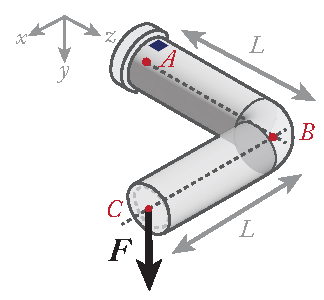
\includegraphics[scale=1]{instr-figures/L-bracket.pdf}
    \caption*{Figure 4.3a.}
    \label{fig:Lbracket}
\end{wrapfigure}
A one-piece polymeric member \textit{ABC} consists of two segments of length $L$ at a right angle from one-another and encastred at $A$, as shown. 
Its neutral axes both lie in the $x-z$ plane when unloaded. 
Assuming the creep compliance in shear to be $\mu_c(t)$ and the creep compliance in axial tension to be $E_c(t)$, determine (a) the deflection at $C$ in terms of the time-varying force $F(t)$ and (b) the stress tensor $\mathbf{\sigma}(t)$ at the square surface element located above $A$.

Let's first define the following quantities for a circular cross-section of radius $r$, area
$$
A = \pi r^2,
$$
second moment of area
$$
I = \frac{\pi r^4}{4},
$$
and torsional constant
$$
J = \frac{\pi r^4}{2},
$$

Because the load at $C$ produces:
\begin{itemize}
    \item bending in the horizontal leg $BC$, and
    \item torsion in the vertical leg $AB$,
\end{itemize}
the total deflection at $C$ is the sum of (i) bending of $BC$ and (ii) torsional rotation of $AB$,
converted into a transverse displacement.

% ---------------------------------------------------
\subsubsection*{(a) Deflection at $C$}

\paragraph{Bending of the segment $BC$}

The straight segment $BC$ behaves as a cantilever beam of length $L$ with a tip load $F(t)$.
The elastic benchmark for a cantilever with tip force $F$ is
$$
\delta_{\max}
=
\frac{F L^{3}}{3 E I}.
$$

To generalize this to a viscoelastic solid, we replace the elastic modulus $E$ by the
creep compliance $E_c(t)$ through the convolution form of Boltzmann superposition.
Thus, the bending deflection at $C$ is
$$
u_C^{(\text{bending})}(t)
=
\frac{L^{3}}{3 I}
\int_{0}^{t}
E_c(t-\tau)\,\frac{dF(\tau)}{d\tau}\,d\tau.
$$

% ---------------------------------------------------
\paragraph{Torsion of the segment $AB$}

The force at $C$ also produces a torque about the axis of segment $AB$.
The moment arm is the length $L$ of the horizontal segment $BC$, so the torque is
$$
T(t) = F(t)\,L.
$$

The correct elastic angle of twist for a circular prismatic bar is
$$
\phi = \frac{T L}{J G},
$$
where $J = \pi r^{4}/2$ is the torsional constant.

To generalize to a viscoelastic material using the shear creep compliance $\mu_c(t)$, we use  
Boltzmann superposition for torsion:
$$
\phi(t)
=
\frac{L^{2}}{J}
\int_{0}^{t}
\mu_c(t-\tau)\,\frac{dF(\tau)}{d\tau}\,d\tau.
$$

Point $C$, located at radius $r$ from the torsional axis, undergoes a transverse displacement
due to this rotation:
$$
u_C^{(\text{torsion})}(t)
=
r \,\phi(t)
=
\frac{r L^{2}}{J}
\int_{0}^{t}
\mu_c(t-\tau)\,\frac{dF(\tau)}{d\tau}\,d\tau.
$$


% ---------------------------------------------------
\paragraph{Total deflection at $C$}

The deflection of point $C$ is the sum of bending of the horizontal segment and the torsional
rotation of the vertical segment:
$$
u_C(t)
=
\frac{L^{3}}{3 I}
\int_{0}^{t}
E_c(t-\tau)\,\frac{dF(\tau)}{d\tau}\,d\tau
+
\frac{r L^{2}}{J}
\int_{0}^{t}
\mu_c(t-\tau)\,\frac{dF(\tau)}{d\tau}\,d\tau.
$$

% ---------------------------------------------------
\subsubsection*{(b) Stress tensor at the square surface above $A$}

We work in a local orthonormal basis attached to the segment $AB$:
$$
\bm{e}_1 \text{ along the z axis},\quad
\bm{e}_2 \text{ along the -y axis},\quad
\bm{e}_3 = \bm{e}_1 \times \bm{e}_2.
$$

The internal resultants at the fixed end $A$ due to the tip force $F(t)$ are, for this
L-shaped bracket,
$$
V(t) = F(t), \qquad
M(t) = F(t)\,L, \qquad
T(t) = F(t)\,L,
$$

\begin{itemize}
  \item \textbf{Normal (bending) stress} at a point a distance $y$ from the neutral axis
  in the $\bm{e}_2$ direction:
  $$
  \sigma_{11}^{(\text{bend})}(t)
  = -\,\frac{M(t)\,y}{I}.
  $$
  At the outer fiber of the surface element above $A$ we have $y = r$, so
  $$
  \sigma_{11}^{(\text{bend})}(t)
  = -\,\frac{F(t)\,L\,r}{I}.
  $$

  \item \textbf{Shear stress from torsion} at radius $r$ in the $\bm{e}_3$ (circumferential)
  direction:
  $$
  \tau_{13}^{(\text{torsion})}(t)
  = \frac{T(t)\,r}{J}
  = \frac{F(t)\,L\,r}{J}.
  $$

  \item \textbf{Shear stress from transverse F} at point A in the $\bm{e}_2$ direction:
  $$
  \tau_{12}^{(\text{transverse force})}(t)
  = \frac{V(t)\,Q}{It}
  = 0.
  $$
  , as $Q$ is 0 at the surface.
\end{itemize}

The non-zero components of the Cauchy stress tensor in the
local basis $\{\bm{e}_1,\bm{e}_2,\bm{e}_3\}$ at the outer surface point are
$$
\sigma_{11}(t) = -\,\frac{F(t)\,L\,r}{I}, \qquad
\sigma_{13}(t) = \sigma_{31}(t) = \frac{F(t)\,L\,r}{J}.
$$

Thus the stress tensor can be written as
$$
\bm{\sigma}(t)
=
\sigma_{11}(t)\,\bm{e}_1\otimes\bm{e}_1
+
\tau_{13}(t)\,\big(
\bm{e}_1\otimes\bm{e}_3
+
\bm{e}_3\otimes\bm{e}_1
\big)
$$

\newpage
\subsection*{4--4. \textbf{Fibrous material} [4 pts].}
An elastic material with a fiber phase has the Helmholtz free energy function
\begin{equation*}
\widetilde{\psi}(\bn{F}) = \frac{1}{2}C_{10} (I_1-3) + \frac{1}{4} k (I_a - 1)^2,
\end{equation*}
where $I_1(\bn{C}) = \textrm{tr}(\bn{C})$ and $I_a(\bn{C},\hat{\bm{a}}_0) = \hat{\bm{a}}_0 \cdot \bn{C} \hat{\bm{a}}_0$ for $\bn{C} = \bn{F}^\intercal \bn{F}$.

%\skiponeline
%(a) Show that, given the direction $\hat{\bm{a}}_0$ is fixed by the material, $I_a$ is an invariant of $\bn{C}$.

\medskip
(a) Show that this elastic potential is consistent with the principle of objectivity.

A superposed rigid rotation $\mathbf{Q}\in\mathrm{SO}(3)$ gives
$$
\mathbf{F}^\ast=\mathbf{Q}\mathbf{F},\qquad
\mathbf{C}^\ast=(\mathbf{F}^\ast)^\top\mathbf{F}^\ast
=\mathbf{F}^\top\mathbf{Q}^\top\mathbf{Q}\mathbf{F}
=\mathbf{F}^\top\mathbf{F}=\mathbf{C}.
$$
Thus
$$
I_1(\mathbf{C}^\ast)=I_1(\mathbf{C}),\qquad
I_a(\mathbf{C}^\ast,\hat{\mathbf{a}}_0)=\hat{\mathbf{a}}_0\cdot\mathbf{C}^\ast\hat{\mathbf{a}}_0
=\hat{\mathbf{a}}_0\cdot\mathbf{C}\hat{\mathbf{a}}_0=I_a(\mathbf{C},\hat{\mathbf{a}}_0),
$$
because $\hat{\mathbf{a}}_0$ is fixed in the material (reference) frame. Hence
$$
\widetilde{\psi}(\mathbf{Q}\mathbf{F})=\widetilde{\psi}(\mathbf{F}),
$$
so the potential is objective.

\medskip
(b) Show that the material symmetry group $\mathcal{G}$ is the set of all proper orthogonal tensors $\bn{H}$ with $\bn{H}\hat{\bm{a}}_0 = \hat{\bm{a}}_0$.  

A right symmetry $\mathbf{H}$ must satisfy
$$
\widetilde{\psi}(\mathbf{F}\mathbf{H})=\widetilde{\psi}(\mathbf{F})\quad\forall\,\mathbf{F}.
$$
For $\mathbf{F}\mathbf{H}$,
$$
\mathbf{C}'=(\mathbf{F}\mathbf{H})^\top (\mathbf{F}\mathbf{H})
=\mathbf{H}^\top \mathbf{C}\,\mathbf{H}.
$$
Then
$$
I_1(\mathbf{C}')=\mathrm{tr}(\mathbf{H}^\top \mathbf{C}\mathbf{H})
=\mathrm{tr}(\mathbf{C}\mathbf{H}\mathbf{H}^\top)=\mathrm{tr}\,\mathbf{C}=I_1(\mathbf{C}),
$$
for any $\mathbf{H}\in\mathrm{SO}(3)$.
For $I_a$,
$$
I_a'=\hat{\mathbf{a}}_0\cdot\mathbf{C}'\hat{\mathbf{a}}_0
=\hat{\mathbf{a}}_0\cdot\mathbf{H}^\top \mathbf{C}\mathbf{H}\hat{\mathbf{a}}_0
=(\mathbf{H}\hat{\mathbf{a}}_0)\cdot\mathbf{C}(\mathbf{H}\hat{\mathbf{a}}_0).
$$
For $I_a'=I_a$ for \emph{all} $\mathbf{C}$, we require
$$
\mathbf{H}\hat{\mathbf{a}}_0 = \hat{\mathbf{a}}_0.
$$
Thus the material symmetry group is
$$
\displaystyle
\mathcal{G}
=\left\{\mathbf{H}\in\mathrm{SO}(3)\ \big|\ \mathbf{H}\hat{\mathbf{a}}_0=\hat{\mathbf{a}}_0\right\},
$$
i.e. all rotations about the fiber direction $\hat{\mathbf{a}}_0$ (transverse isotropy).

\medskip
(c) Find the first Piola-Kirchhoff and Cauchy stress expressions with an applied deformation gradient tensor of $\bn{F}$.

First compute
$$
\frac{\partial I_1}{\partial\mathbf{C}}=\mathbf{I},\qquad
\frac{\partial I_a}{\partial\mathbf{C}}=\hat{\mathbf{a}}_0\otimes\hat{\mathbf{a}}_0.
$$
Then
$$
\frac{\partial\widetilde{\psi}}{\partial\mathbf{C}}
= \frac12 C_{10}\,\mathbf{I}
+ \frac14 k\cdot 2(I_a-1)(\hat{\mathbf{a}}_0\otimes\hat{\mathbf{a}}_0)
= \frac12 C_{10}\,\mathbf{I}
+ \frac12 k(I_a-1)(\hat{\mathbf{a}}_0\otimes\hat{\mathbf{a}}_0).
$$
So the second Piola–Kirchhoff stress is
$$
\mathbf{S} = 2\,\frac{\partial\widetilde{\psi}}{\partial\mathbf{C}}
= C_{10}\,\mathbf{I}+k(I_a-1)(\hat{\mathbf{a}}_0\otimes\hat{\mathbf{a}}_0).
$$

The first Piola–Kirchhoff stress is
$$
\displaystyle
\mathbf{P} = \mathbf{F}\,\mathbf{S}
= \mathbf{F}\Big[ C_{10}\,\mathbf{I}+k(I_a-1)(\hat{\mathbf{a}}_0\otimes\hat{\mathbf{a}}_0)\Big].
$$

Let
$$
\mathbf{a} = \mathbf{F}\hat{\mathbf{a}}_0,\qquad
\mathbf{B}=\mathbf{F}\mathbf{F}^\top,\qquad
J=\det\mathbf{F}.
$$
The Cauchy stress is
$$
\boldsymbol{\sigma} = \frac{1}{J}\,\mathbf{P}\mathbf{F}^\top
= \frac{1}{J}\Big[C_{10}\,\mathbf{B}
+ k(I_a-1)(\mathbf{a}\otimes\mathbf{a})\Big].
$$

For an incompressible material ($J=1$) with Lagrange multiplier $p$, it should be added $-p\mathbf{I}$:
$$
\displaystyle
\boldsymbol{\sigma}
= C_{10}\,\mathbf{B}
+ k(I_a-1)(\mathbf{a}\otimes\mathbf{a})
- p\,\mathbf{I}.
$$

\bigskip
\bigskip
\subsection*{4--5. \textbf{Gent model of rubber elasticity} [4 pts].}
The Gent model, which incorporates the finite extensibility of polymer chains in a rubber network but includes $I_2$-dependence, has a\textcolor{red}{n isochoric} free-energy function of $$\bar{\Psi}_{\textcolor{red}{\textrm{iso}}} = -\frac{C_{10}}{2} J_m \ln \left(1 - \frac{I_1-3}{J_m} \right) + C_{01}\ln \left(\frac{I_2}{3}\right), $$ where $C_{10}>0$, $C_{01}\geq 0$, and $J_m>0$ are material constants.

\medskip
(a) Show that the Cauchy stress corresponding to the free energy above has the form\footnote{\textcolor{red}{You may want to use the Cayley-Hamilton theorem to do a replacement for $\bn{B}^2$, which produces $\bn{B}^2 = I_1 \bn{B} - I_2 \bn{I} + I_3 \bn{B}^{-1}$.}} $$\bm{\sigma} = -p \bn{I} + \frac{C_{10} J_m}{J_m - (I_1-3)}\bn{B} - \frac{2C_{01}}{I_2} \bn{B}^{-1}.$$

For an incompressible isotropic solid, the Cauchy stress is
$$
\boldsymbol{\sigma}
= -p\,\mathbf{I}
+ 2\frac{\partial\bar{\Psi}_{\mathrm{iso}}}{\partial I_1}\mathbf{B}
- 2\frac{\partial\bar{\Psi}_{\mathrm{iso}}}{\partial I_2}\mathbf{B}^{-1},
$$

Compute
$$
\frac{\partial\bar{\Psi}_{\mathrm{iso}}}{\partial I_1}
= -\frac{C_{10}}{2}J_m\cdot
\frac{1}{1-\frac{I_1-3}{J_m}}\left(-\frac{1}{J_m}\right)
= \frac{C_{10}}{2}\frac{J_m}{J_m-(I_1-3)},
$$
and
$$
\frac{\partial\bar{\Psi}_{\mathrm{iso}}}{\partial I_2}
= C_{01}\cdot\frac{1}{I_2}.
$$
Therefore
$$
\boldsymbol{\sigma}
= -p\,\mathbf{I}
+ 2\left(\frac{C_{10}}{2}\frac{J_m}{J_m-(I_1-3)}\right)\mathbf{B}
- 2\left(\frac{C_{01}}{I_2}\right)\mathbf{B}^{-1},
$$
so
$$
\displaystyle
\boldsymbol{\sigma}
= -p\,\mathbf{I}
+ \frac{C_{10}J_m}{J_m-(I_1-3)}\,\mathbf{B}
- \frac{2C_{01}}{I_2}\,\mathbf{B}^{-1}.
$$

\medskip
(b) This material undergoes a simple shear deformation of magnitude $\gamma$. Given that the shear modulus $\mu(\gamma^2) \equiv \beta_1(\gamma^2) - \beta_{-1} (\gamma^2)$ where $\beta_i$ corresponds to the expression for $\bm{\sigma}$ in Q1, show that in the small strain limit that $$\lim\limits_{\gamma \rightarrow 0} \mu(\gamma^2) = C_{10} + \frac{2}{3} C_{01}.$$

Consider simple shear of magnitude $\gamma$:
$$
\mathbf{F} =
\begin{pmatrix}
1 & \gamma & 0\\
0 & 1 & 0\\
0 & 0 & 1
\end{pmatrix},
\qquad
\mathbf{B}=\mathbf{F}\mathbf{F}^\top
=
\begin{pmatrix}
1+\gamma^2 & \gamma & 0\\
\gamma & 1 & 0\\
0 & 0 & 1
\end{pmatrix}.
$$
Then
$$
I_1 = 3+\gamma^2,\qquad
I_2 = 3+\gamma^2
$$
for this deformation.

We can write the Cauchy stress in the standard representation
$$
\boldsymbol{\sigma}
= -p\,\mathbf{I}
+ \beta_1(\gamma^2)\,\mathbf{B}
- \beta_{-1}(\gamma^2)\,\mathbf{B}^{-1},
$$
where, by comparison with part (a),
$$
\beta_1(\gamma^2) = \frac{C_{10}J_m}{J_m-(I_1-3)}
= \frac{C_{10}J_m}{J_m-\gamma^2},
\qquad
\beta_{-1}(\gamma^2) = \frac{2C_{01}}{I_2}
= \frac{2C_{01}}{3+\gamma^2}.
$$

Evaluate at $\gamma=0$:
$$
\beta_1(0) = \frac{C_{10}J_m}{J_m} = C_{10},\qquad
\beta_{-1}(0) = \frac{2C_{01}}{3}.
$$
So
$$
\displaystyle
\lim_{\gamma\to 0}\mu(\gamma^2)
= C_{10}+\frac{2}{3}C_{01}.
$$
%\setcounter{section}{3} % This causes the next section to be Appendix B


\section*{Examples III. Linear Viscoelastic Models}
\label{PS3}

This set of example problems is due on October 17, 2025. 

% This is a placeholder for the example problems from the third problem set. 
% You'll replace this file with the one I supply on canvas. 

\medskip
\subsection*{3--1. \textbf{Converting creep to relaxation} [4 pts].} 
Say we measure the creep function for a material by fitting a sum of exponential functions to some data. 
We determine the creep function to be 
\begin{equation}
    J_c(t) = \frac{1}{1000}\left(10 - 5 e^{-t/4} - 3e^{-t/8}\right).
\end{equation}
(a) Attach a plot of $J_c(t)$, labeling significant values.
Significant values: $$J_c(0^+) = 2\times 10^{-3}\ {\rm Pa^{-1}},\qquad J_c(\infty)=10\times 10^{-3}\ {\rm Pa^{-1}}.$$ 
The characteristic \emph{creep} times from the fit are $$\tau_{c1}=4~{\rm s},\qquad \tau_{c2}=8~{\rm s}.$$

\begin{figure}[H]
\centering
\includegraphics[width=0.66\textwidth]{fig_PS3_Jc.png}
\caption{\small Creep compliance $J_c(t)$.}
\end{figure}

(b) Determine the corresponding stress relaxation function $G_r(t)$. What are the characteristic stress relaxation times now, and how do they compare to the creep relaxation times? 
For linear viscoelasticity,
$$
\big[s\,J_c(s)\big]\big[s\,G_r(s)\big]=1
\quad\Longleftrightarrow\quad
G_r(s)=\frac{1}{s^2 J_c(s)}.
$$
Laplace transforming
$$
J_c(t)=\frac{1}{1000}\left(10 - 5 e^{-t/4} - 3e^{-t/8}\right)
\ \Longrightarrow\
J_c(s)=\frac{1}{100}\frac{1}{s}-\frac{1}{200}\frac{1}{s+\tfrac{1}{4}}-\frac{3}{1000}\frac{1}{s+\tfrac{1}{8}}.
$$
Algebra gives
$$
J_c(s)=\frac{32s^2+38s+5}{500\,s\,(32s^2+12s+1)},\qquad
G_r(s)=\frac{500(32s^2+12s+1)}{s\,(32s^2+38s+5)}.
$$
In time domain,
$$
G_r(t)=100\;+\;A\,e^{s_1 t}\;+\;B\,e^{s_2 t},
$$
where
$$
s_{1,2}=\frac{-19\pm\sqrt{201}}{32}
\ \Rightarrow\
\tau_{r1}=\frac{1}{|s_1|}\approx 0.9645~{\rm s},\quad
\tau_{r2}=\frac{1}{|s_2|}\approx 6.634~{\rm s},
$$
and
$$
A=200+\frac{900}{67}\sqrt{201}\approx 390.44,\qquad
B=200-\frac{900}{67}\sqrt{201}\approx 9.56.
$$
Thus a single Prony form:
$$
G_r(t)=100\;+\;390.44\,e^{-t/0.9645}\;+\;9.56\,e^{-t/6.634}\quad[{\rm Pa}].
$$
\emph{Comparison:} the \emph{relaxation} times $$\tau_{r1}\approx 0.9645~{\rm s},\ \ \tau_{r2}\approx 6.634~{\rm s}$$ 
differ from the creep times 4 and 8 s; this is expected because $J_c$ and $G_r$ are convolution inverses rather than sharing identical time constants.

\bigskip
\bigskip
\bigskip
\subsection*{3--2. \textbf{Alternate standard linear solid model} [4 pts].}

In class, we derived the relaxation and creep compliance functions $G_r(t)$ and $J_c(t)$ for a standard linear solid (SLS) model consisting of a spring in parallel with a Maxwell branch. 
In this question, we'll investigate a variant arrangement for the SLS, where a spring is placed in series with a Kelvin-Voigt solid. 

(a) Determine the differential constitutive law for the variant SLS. 
$$
\sigma=\sigma_s=\sigma_{kv},\qquad \varepsilon=\varepsilon_s+\varepsilon_{kv}.
$$
Elements:
$$
\sigma=E_s\,\varepsilon_s,\qquad \sigma=E_k\,\varepsilon_{kv}+\eta_k\,\dot\varepsilon_{kv}.
$$
Eliminate strains using
$$\varepsilon=\sigma/E_s+\varepsilon_{kv}$$ differentiate, and rearrange to obtain
$$
\ \dot\sigma+\frac{E_s+E_k}{\eta_k}\,\sigma
= E_s\,\dot\varepsilon+\frac{E_sE_k}{\eta_k}\,\varepsilon.\
$$
(b) Then, the creep compliance function $J_c(t)$ and hence, the relaxation function $G_r(t)$.

Compliances add in series. KV creep:
$$
J_{kv}(t)=\frac{1}{E_k}\Big(1-e^{-t/\tau_c}\Big),\qquad \tau_c=\frac{\eta_k}{E_k}.
$$
Therefore
$$
\ J_c(t)=\frac{1}{E_s}+\frac{1}{E_k}\Big(1-e^{-t/\tau_c}\Big)
=\Big(\frac{1}{E_s}+\frac{1}{E_k}\Big)-\frac{1}{E_k}e^{-t/\tau_c}\ .
$$
Using $\big[sJ_c(s)\big]\big[sG_r(s)\big]=1$, one finds
$$
\ G_r(t)=G_\infty + (G_0-G_\infty)\,e^{-t/\tau_r},\quad
G_0=E_s,\ \ G_\infty=\frac{E_sE_k}{E_s+E_k},\ \ \tau_r=\frac{\eta_k}{E_s+E_k}.\
$$
(c) How do the coefficients in the two variants of the standard solid model relate to each other?

$$
E_s=E_p+E_m,\quad
E_k=\frac{E_pE_s}{E_m},\quad
\eta_k=\frac{(E_p+E_m)^2}{E_m^2}\,\eta_m\;
$$
and the inverse
$$
\
E_m=\frac{E_s^2}{E_s+E_k},\quad
E_p=\frac{E_sE_k}{E_s+E_k},\quad
\eta_m=\frac{E_s^2}{(E_s+E_k)^2}\,\eta_k\ .
$$
\bigskip
\bigskip
\bigskip
\subsection*{3--3. \textbf{Frequency response of a 5-term analog model} [4 pts].}
You have a five-parameter fit $G_r(t) = C_r (200 e^{-2t} + 100 e^{-t} + 10)$ that describes the relaxation behavior of a real material. 

(a) Draw the equivalent mechanical analog model for this fit.

\begin{figure}[H]
\centering
\includegraphics[width=0.66\textwidth]{fig_PS3_analog.png}
\caption{\small Mechanical analog model.}
\end{figure}

(b) Determine the functional forms for the storage and loss moduli, and create a semi-log plot of the loss tangent $(\tan\delta)$ over a domain of relevant frequency orders $(\log \omega)$. 

For a generalized Maxwell model,
$$
G'(\omega)=E_\infty+\sum_k\frac{E_k(\omega\tau_k)^2}{1+(\omega\tau_k)^2},\qquad
G''(\omega)=\sum_k\frac{E_k(\omega\tau_k)}{1+(\omega\tau_k)^2}.
$$
Hence
$$
G'(\omega)=10C_r+200C_r\,\frac{(\omega/2)^2}{1+(\omega/2)^2}
+100C_r\,\frac{\omega^2}{1+\omega^2},
$$
$$
G''(\omega)=100C_r\,\frac{\omega}{1+(\omega/2)^2}
+100C_r\,\frac{\omega}{1+\omega^2},\qquad
\tan\delta(\omega)=\frac{G''(\omega)}{G'(\omega)}.
$$

\begin{figure}[H]
\centering
\includegraphics[width=0.66\textwidth]{fig_PS3_tandelta.png}
\caption{\small Semi-log plot of loss tangent $\tan\delta(\omega)$ vs. $\omega$ for the given Prony fit.}
\end{figure}

\newpage
\subsection*{3--4. \textbf{Fractional response} [4 pts].}

This question will be best approached numerically, using e.g. Matlab or Mathematica. 

Fractional order models can be used to show relaxation that does not follow the classic ``S-curve'' Debye relaxation function for $G_r(t)$ vs. $\log t$. 

Starting from a Kelvin-Voigt-type fractional model with the functional form of 
\begin{equation*}
    G_r(t) = \left[10 + 2\left(\frac{t}{0.2} \right)^{-\alpha}\right] \mathcal{H}(t),
\end{equation*}
plot the stress and strain responses of this solid over time (i.e., plot $\sigma(t,\alpha)$ and $\varepsilon(t,\alpha)$ on separate plots for each part) for a range of values of $0<\alpha<1$ to (a) a step strain, (b) a step stress of only length $t=5$, and (c) another stress function entirely of your choice. 

As a suggestion, you could consider values spaced symmetrically around zero on the logistic distribution, which is defined as $\textrm{logit}(\alpha) = \log\left(\frac{\alpha}{1-\alpha} \right)$. 
Picking e.g., logit($\alpha$)$=0$ corresponds to $\alpha =0.5$, $\textrm{logit}(\alpha) =  1$ is $\alpha\approx0.73$, etc. 
I suggest sampling integers on a range of logit($\alpha$) $= -4 \textrm{~to~} 4$ to cover the full range from elastic to viscous response for the springpot.

\paragraph{(a) Step strain}
For $\varepsilon(t)=\varepsilon_0\mathcal{H}(t)$, the stress response is
$$
\sigma(t,\alpha)=\varepsilon_0\,G_r(t).
$$
A representative plot is shown below.

\paragraph{(b) Finite step stress of length $t=5$}
We solve
$$
E\,\varepsilon(t)+\eta_\alpha\,{}^{C}D_t^\alpha \varepsilon(t)=\sigma_0\,[\mathcal{H}(t)-\mathcal{H}(t-5)]
$$

\paragraph{(c) Another stress: half-sine pulse on $0\le t\le 10$.}
We solve the same fractional KV equation with
$$
\sigma(t)=\sigma_0\sin\!\Big(\frac{\pi t}{10}\Big)\, \mathcal{H}(t)\,\mathcal{H}(10-t).
$$

\begin{figure}[H]
\centering
\subfigure[\small Stress responses $\sigma(t,\alpha)$ for step strain $\epsilon=\epsilon_0 \mathcal{H}(t)$.]{
  \includegraphics[width=0.85\textwidth]{fig_PS3_frac_stepstrain_sigma.png}
}
\quad
\subfigure[\small Applied strain history (constant step).]{
  \includegraphics[width=0.85\textwidth]{fig_PS3_frac_stepstrain_eps.png}
}
\caption{\small Fractional Kelvin--Voigt: step strain responses for multiple $\alpha$.}
\end{figure}

\begin{figure}[H]
\centering
\subfigure[\small Strain responses $\epsilon(t,\alpha)$ for finite step stress ($0\le t<5$ s).]{
  \includegraphics[width=0.85\textwidth]{fig_PS3_frac_stepstress_eps.png}
}
\quad
\subfigure[\small Applied stress $\sigma(t)$ used for part (b).]{
  \includegraphics[width=0.85\textwidth]{fig_PS3_frac_stepstress_sigma.png}
}
\caption{\small Fractional Kelvin--Voigt: finite step stress of length $5$ s.}
\end{figure}

\begin{figure}[H]
\centering
\subfigure[\small Strain responses $\epsilon(t,\alpha)$ for half-sine stress on $0\le t\le 10$ s.]{
  \includegraphics[width=0.85\textwidth]{fig_PS3_frac_halfsine_eps.png}
}
\quad
\subfigure[\small Applied half-sine stress $\sigma(t)$ used for part (c).]{
  \includegraphics[width=0.85\textwidth]{fig_PS3_frac_halfsine_sigma.png}
}
\caption{\small Fractional Kelvin--Voigt: half-sine stress case.}
\end{figure}


\bigskip
\bigskip
\subsection*{3--5. \textbf{Rheology without a rheometer} [8 pts].}

You have a rubbery material of density $\rho$ for which you plan to characterize frequency-dependent viscoelastic behavior. 
The material you have can be made into a sphere of a wide range of sizes, from a radius of $R=1$ mm to $R=1$ m. 
You plan to drop each ball onto a rigid half-space from a height $h_0$, and can measure the height $h(R)$ for each ball radius $R$. 

The impact duration for an elastic material is given by a Hertzian contact relation of
\begin{equation*}
    t_c = 5.21\frac{R}{c}\left(\frac{c}{\sqrt{2 g h_0}}\right)^{1/5} \approx 0.025R  \textrm{~~[s]}
\end{equation*}
where $c = 1000$ m/s represents the pressure wave speed in the material and the initial height $h_0$ is taken to be a consistent 0.01 m.

(a) How much energy per volume is dissipated by the material for each size of ball? 

With drop height $h_0$ and rebound height $h(R)$, the dissipated energy per unit volume is
$$
\Delta w(R)=\rho g\,\big[h_0-h(R)\big]. 
$$

(b) Using the Lissajous plot of $\sigma/|E^*|$ vs. $\varepsilon$, show that the approximate peak elastic energy stored in the ball during a half-cycle is $\frac{1}{2} B^2 \cos \delta$, where $B = \varepsilon_{\textrm{max}}$. 

Normalize the stress by $|E^*|$ and plot $\sigma/E,\varepsilon$.
For sinusoidal steady response $\varepsilon=B\sin\omega t$ and $\sigma=|E^*|\,B\sin(\omega t+\delta)$, the peak elastic energy density in a half-cycle is
$$
w_{\rm el,peak}\approx \frac{1}{2}\,B^2\cos\delta\ \times |E^*|.
$$

(c) Determine an approximate expression for the energy dissipated by the ball during a drop event in terms of $A = \varepsilon_{\textrm{max}} \sin \delta$ and $B$. 

The Lissajous ellipse area per full cycle is $\pi |E^*| AB$, where $A=B\sin\delta$.
A single impact spans roughly a half-cycle, so
$$
\ \Delta w_{\rm half}\approx \frac{\pi}{2}\,|E^*|\,A\,B
= \frac{\pi}{2}\,|E^*|\,AB.\
$$

(d) Hence, determine $\tan\delta$ as a function of the rebound height, $h(R)$. 

Using the ratio of dissipated to peak elastic energy in a half-cycle,
$$
\frac{\Delta w_{\rm half}}{w_{\rm el,peak}}\ \approx\ \pi\,\tan\delta.
$$
Assuming the total dissipated energy in the drop equals the gravitational loss per volume,
$$
\Delta w(R)=\rho g\,[h_0-h(R)]\ \approx\ 2\,\Delta w_{\rm half},
$$
Assuming the peak elastic energy reflect the potential energy at the maximum height,
$$
w_{\rm el,peak} =\rho g\,h(R),
$$
so
$$
\tan\delta \ \approx\ \frac{1}{\pi}\,\frac{\Delta w_{\rm half}}{w_{\rm el,peak}}
\ \approx\ \frac{1}{2\pi}\,\frac{\,[h_0-h(R)]}{h(R)}.
$$

(e) For what frequencies could you say this material is calibrated?

With $R\in[1~{\rm mm},\,1~{\rm m}]$,
$$
t_c\in[2.5\times 10^{-5},\ 2.5\times 10^{-2}]~{\rm s},\qquad
f_c\sim \frac{1}{2t_c}\in[20,\ 2\times 10^{4}]~{\rm Hz}.
$$
Thus the drop tests effectively probe $\sim 20~{\rm Hz}$ to $20~{\rm kHz}$ across the available radii.
%\setcounter{section}{1} % This causes the next section to be Appendix B

\section{Kinetics, Constitutive Laws, and Viscoelasticity I}
\label{PS2}

This set of example problems is due on October 3, 2025. 
As before, I request that you type up your responses in \LaTeX~ rather than write them out by hand. 

\medskip
\subsection*{2--1. \textbf{Balance of mass} [4 pts].} 
A large piece of polydimethylsiloxane (PDMS) of uniform density $\rho(\bm{x},t)$ has a central spherical bubble of time-evolving radius $R(t)$, initial radius $R_0$, and wall velocity of $\dot{R}$. 
The hole is subject to a uniform surface traction in the $\bm{e}^{(r)} \equiv \bm{e}_{\bm{r}}$ direction from an axisymmetric pressure, and maintains spherical symmetry over time. 

\medskip
The position of a point in the material can be written as $\bm{x} = r(R,t) \bm{e}_{\bm{r}}$ with reference position $\bm{X} = r_0(R_0)$, while the velocity of that point can be written as $\bm{v}(r,t) = v_r \bm{e}_{\bm{r}}$.

\medskip
Using the conservation of mass equation, show that the material must satisfy
%\begin{equation}
%\rho_{,t} + (\rho v_i)_{,i} = 0,
%\end{equation}
\begin{equation*}
\rho_{,t}+ \rho_{,r} v_r + \frac{\rho}{r} (v_r + r v_{r,r}) = 0,
\end{equation*}
and hence, show that an assumption of incompressibility for PDMS results in 
\begin{equation*}
v_r(r,t) = \frac{R^2 \dot{R}}{r^2}.
\end{equation*}

\medskip
\subsection*{2--2. \textbf{Balance of momenta} [4 pts].} A spherical hydrogel body $\mathcal{B}$ with a linear density gradient is currently submerged in water as depicted in the figure. 
The sphere has coordinates $\bm{x}$ in a region $\Omega$ with position-dependent density $\rho(\bm{x})$. 

\begin{figure}[H]
\vspace{-2em}
\centering
\includegraphics[width=3in]{instr-figures/PS2-Q1.pdf}  
\caption{\small{Hydrogel sphere with a linear density gradient submerged in water. The water has a density $\rho_w$, while the sphere has a density at its leftmost point of $\rho_w/2$ and at its rightmost point of $3\rho_w/2$.}}
\end{figure}

\vspace{-1em}
The surface traction $\bm{t}(\bm{x},\hat{\bm{n}})$ acting on $\mathcal{B}$ is given by 
\begin{equation*}
\bm{t}(\bm{x},\hat{\bm{n}}) = -\rho_w g x_3 \hat{\bm{n}},
\end{equation*}
where $\hat{\bm{n}}$ is the outer unit normal to the surface $\partial \Omega_t$ and $\rho_w$ is the (constant) density of water and $g$ is the acceleration due to gravity. 

\medskip
(a) Determine the net force and moment acting on $\mathcal{B}$ via volume integrals.

\medskip
(b) Under what \textit{two} conditions is $\mathcal{B}$ in static equilibrium?


% \subsection*{2--1. \textbf{Balance of momentum} [4 pts].} A Cauchy stress field in a material has a matrix of scalar components in the 3D basis $\{\bn{e}_i\}$:
% \begin{equation}
% \bm{\sigma} = \begin{bmatrix}
% 4x_1 x_3 & 0 & -2 x_3^2 \\
% 0 & 1 & 2 \\
% -2 x_3^2 & 2 & 3 x_1^2
% \end{bmatrix} \textrm{~(MPa)}
% \end{equation}
% where the material originally on a domain $\bm{X} \in \Omega_0$ is mapped to a new domain $\bm{x}\in \Omega$ (with units of meters). 

% \medskip
% (a) For the static case with no applied body force, is this stress field in equilibrium?

% \medskip
% (b) At a position vector $\bm{x}_1 = 2\bm{e}_1 +  \bm{e}_2 + \bm{e}_3 $, determine the traction, $\bm{t}$, caused by the stress tensor at a cut plane given by the equation $x_1 + x_2 - x_3 = 2$. 

% \medskip
% (c) Find the magnitudes of the shear and normal traction on this plane at the point $\bm{x}_1$. 

% \medskip
% (d) Computationally determine the principal stresses and associated directions at the given point. Why, in general, can a principal stress be negative but a principal stretch cannot?


\bigskip
\subsection*{2--3. \textbf{Viscoelastic data} [4 pts].} 
Stress relaxation isochrones for a compliant viscoelastic material are shown in the figure below.  

\begin{figure}[H]
\vspace{-1em}
\centering
\includegraphics[scale = 1.5]{instr-figures/PS2-Q3.pdf}
\caption{\small{Stress (Pa) vs. strain ($-$) for a soft viscoelastic material.}}
\end{figure}

\vspace{-1em}
(a) Are these isochrones from a material which we can describe with linear viscoelasticity? If not, why not, and if so, under what approximate regimes would this assumption be valid? 

\medskip
(b) Estimate the creep relaxation function $J_c$ for stress values of 100 and 250 kPa. Isochrones are shown at times of 2, 5, 10, 20, and 40 seconds.   
% This is a placeholder for the example problems from the second problem set. 
% You'll replace this file with the one I supply on canvas. 

\bigskip
\subsection*{2--4. \textbf{Impulsive stresses} [4 pts].}

(a) Say that instead of a step load, we apply $\sigma(t) = A \delta(t)$ to an unknown linear viscoelastic material. 
Determine the strain history $\epsilon(t)$, first as a general function of the creep relaxation function $J_c(t)$, and then for a Kelvin-Voigt solid. 

(b) Now, consider a rapid load followed by a rapid reverse load by applying a doublet function of stress, i.e. $\sigma(t) = B \psi(t)$. 
What is the strain function $\epsilon(t)$ in terms of $J_c(t)$ and for a Kelvin-Voigt material now? 


\bigskip
\subsection*{2--5. \textbf{Two-element models} [8 pts].}

Dynamic mechanical analysis (DMA) is a common technique for characterizing viscoelasticity. 
DMA conventionally involves application of a sinusoidal displacement to the top surface of a sample at a controllable temperature. 
Often, the user puts the sample into initial compression, and follows with the sinusoidal profile. 
A cylindrical sample of height $h$ and diameter $d$ is placed between two plates.
The DMA then quickly puts the sample into compression by moving its top plate downward by a displacement $d$, and then oscillates sinusoidally between positions $0$ and $2d$ at a frequency $\omega$.

\medskip
(a) Using the constitutive law for a Kelvin-Voigt material, determine the stress $\sigma(t)$ exerted by the platens to cause the applied strain. 

\medskip
(b) The resulting stress lags behind the strain by an phase $\delta$, as in $\sin(\omega t + \delta)$. 
Commonly this is reported as the ``tangent loss", or $\tan\delta$, for a material. 
What is the value of $\tan\delta$ for this particular Kelvin-Voigt model?

\medskip
(c) Say instead of prescribing the strain $\epsilon(t)$, we instead prescribed the stress, $\sigma(t) = - \sigma_0 - \sigma_0 \sin(\omega t)$. 
Determine the strain $\epsilon(t)$ for this prescribed stress.

\medskip
(d) Prove that the tangent loss function $\tan\delta$ is identical between the two loading methods.






%
\section*{Examples I. Mathematical Preliminaries (due \textcolor{red}{Sept 19})}
\textcolor{red}{(Rev note: v2)}
\label{PS1}

This set of example problems is due on September 17, 2025. 
I request that you type up your responses in \LaTeX~ rather than write them out by hand. 
The primary reason is to become better acquainted with writing up mechanics in archival format. 
If you have diagrams, plots, etc., please add them as attached figures using the \texttt{includegraphics} command. 

\bigskip
\subsection*{1--1. \textbf{Convolutional integrals} [4 pts].} The response of a 1D viscoelastic material to an applied forcing function is given using a convolutional integral:
\begin{equation}
    \varepsilon(t) = \int_0^t J(t-\tau) \frac{d\sigma(\tau)}{d\tau} d\tau,
\end{equation}
where $\varepsilon(t)$ is the time-dependent strain response, $\sigma(t)$ is the prescribed stress function, and $J(t)$ is the material compliance, assumed to not depend on the level of stress applied. 
Say we have a compliance function 
\begin{equation}
    J(t) = J_\infty + (J_0-J_\infty)\exp[-t/\tau_c],
\end{equation}
where $J_0, J_\infty, \tau_c$ are all constants $\in \mathbbm{R}$. 
We subject this material to two different loading profiles: (a) step load $\sigma_1(t) = \sigma_0 H(t)$ and (b) a sinusoidal load $\sigma_2(t) = \sigma_0  \sin(\omega t)$, where $\sigma_0$ and $\omega$ are also constant, and $H(t)$ is the step function. 

Determine the corresponding Laplace transforms of the strain functions $\mathcal{L}\{\varepsilon_1(t)\}$ and $\mathcal{L}\{\varepsilon_2(t)\}$. 

\textit{\textbf{Dare mode:}} If you have taken complex analysis, you can compute the inverse transform of polynomial forms because this type of model yields terms with simple poles (i.e. linear in $s$). 
The formulae for this (see e.g. \cite{rileyMathematicalMethodsPhysics2006} Chs. 24 and 25) are:
\begin{equation*}
    \textrm{Residue for simple poles: } R(f(s),s_0) = \lim\limits_{s\rightarrow s_0} \left[ (s-s_0) f(s) \right],
\end{equation*}
and you multiply each residue by the shift from zero, i.e.,
\begin{equation*}
    f(t) = \mathcal{L}^{-1}\{F(s)\} = \sum \left( \textrm{residues of } F(s)e^{s_0 t} \textrm{ at all poles } s_0 \right)
\end{equation*}
\textit{If you dare}, determine the corresponding strain histories $\varepsilon_1(t)$ and $\varepsilon_2(t)$. The first is relatively straightforward; the latter has complex poles and more terms. 

%\newpage
\bigskip
\textbf{Answer:}
Given
\begin{equation}
  \varepsilon(t)=\int_0^t J(t-\tau)\,\frac{d\sigma(\tau)}{d\tau}\,d\tau,
  \qquad
  J(t)=J_\infty+(J_0-J_\infty)e^{-t/\tau_c},
\end{equation}
its Laplace transform (with $\sigma(0^-)=0$ and using $\mathcal{L}\{f*g\}=F(s)G(s)$,
$\mathcal{L}\{\dot{\sigma}\}=s\varepsilon(s)$) is
\begin{equation}
  E(s)=\mathcal{L}\{\varepsilon(t)\}=J(s)\,s\,\varepsilon(s),
  \qquad
  J(s)=\frac{J_\infty}{s}+\frac{J_0-J_\infty}{\,s+1/\tau_c\,}.
\end{equation}

\paragraph{(a) Step load}
For $\sigma_1(t)=\sigma_0 H(t)$, we have $\varepsilon_1(s)=\sigma_0/s$, hence
\begin{equation}
  \,E_1(s)=\sigma_0\,J(s)=\sigma_0\!\left(\frac{J_\infty}{s}+\frac{J_0-J_\infty}{\,s+1/\tau_c\,}\right).\,
\end{equation}

\paragraph{(b) Sinusoid}
For $\sigma_2(t)=\sigma_0\sin(\omega t)$, we have $\varepsilon_2(s)=\dfrac{\sigma_0\omega}{s^2+\omega^2}$, hence
\begin{equation}
  \,E_2(s)=J(s)\,s\,\Sigma_2(s)
  =\sigma_0\omega\left[\frac{J_\infty}{s^2+\omega^2}
  +\frac{(J_0-J_\infty)\,s}{(s+1/\tau_c)(s^2+\omega^2)}\right].\,
\end{equation}

\bigskip
\subsection*{1--2. \textbf{Index notation} [4 pts].} Let $\bm{p}, \bm{q}, \bm{r}, \bm{a}, \bm{b}$ be vector fields on $\mathbbm{R}^3$ and $\bn{Q}$ be a change-of-basis tensor on $\mathbbm{R}^3$. Show the following identities to be true using index notation. 

\begin{itemize}
    \item $\bm{p} \times (\bm{q} \times \bm{r}) = (\bm{r} \cdot \bm{p}) \bm{q} - (\bm{q} \cdot \bm{p}) \bm{r}$
    \item $(\bm{p} \times \bm{q}) \cdot (\bm{a} \times \bm{b}) = (\bm{p} \cdot \bm{a}) (\bm{q} \cdot \bm{b}) - (\bm{q} \cdot \bm{a})(\bm{p} \cdot \bm{b})$
    \item $(\bm{a} \otimes \bm{b})(\bm{p} \otimes \bm{q}) = \bm{a}\otimes\bm{q}(\bm{b} \cdot \bm{p}) $
    \item $\bn{Q}^\intercal\bm{a} \cdot \bn{Q}^\intercal\bm{b} = \bm{a}\cdot\bm{b} $
\end{itemize}

\bigskip 
\textbf{Answer:}
Use $(\bm{a}\times\bm{b})_i=\varepsilon_{ijk}a_j b_k$ and the identity 
$\varepsilon_{ijk}\varepsilon_{imn}=\delta_{jm}\delta_{kn}-\delta_{jn}\delta_{km}$.

\paragraph{(i)}
\begin{align*}
\big[\bm{p}\times(\bm{q}\times\bm{r})\big]_i 
&= \varepsilon_{ijk}p_j(\varepsilon_{klm}q_l r_m) \\
&= (\delta_{i\ell}\delta_{jm}-\delta_{im}\delta_{j\ell})\,p_j q_\ell r_m \\
&= (p_j r_j)q_i-(p_j q_j)r_i \\
&=((\bm{r}\cdot\bm{p})\,q_i - (\bm{q}\cdot\bm{p})\,r_i).
\end{align*}

\paragraph{(ii)}
\begin{align*}
(\bm{p}\times\bm{q})\cdot(\bm{a}\times\bm{b})
&=\varepsilon_{ijk}p_j q_k\,\varepsilon_{ilm}a_l b_m \\
&=(\delta_{jl}\delta_{km}-\delta_{jm}\delta_{kl})\,p_j q_k a_l b_m \\
&=p_j a_j q_k b_k-p_j b_j q_k a_k\\
&=(\bm{p}\cdot\bm{a})(\bm{q}\cdot\bm{b})-(\bm{p}\cdot\bm{b})(\bm{q}\cdot\bm{a}).
\end{align*}

\paragraph{(iii)}
\begin{align*}
\big[(\bm{a}\otimes\bm{b})(\bm{p}\otimes\bm{q})\big]_{ij}
&=(a_i b_k)(p_k q_j) \\
&=a_i q_j\,(b_k p_k) \\
&=\big(\bm{b}\cdot\bm{p}\big)\,(\bm{a}\otimes\bm{q})_{ij}.
\end{align*}

\paragraph{(iv)}
\begin{align*}
(\bn{Q}^\top\bm{a})\cdot(\bn{Q}^\top\bm{b})
&=(Q_{ki}a_i)(Q_{kj}b_j) \\
&=(Q_{ki}Q_{kj})\,a_i b_j \\
&=\delta_{ij}a_i b_j \\
&=\bm{a}\cdot\bm{b},
\end{align*}
where $\bn{Q}$ is an orthogonal change-of-basis tensor ($Q_{ki}Q_{kj}=\delta_{ij}$).
\bigskip

\subsection*{1--3. \textbf{Tensors and vectors} [4 pts].}
The second-order projection tensors $\bn{P}_{\bm{n}}^{||}$ and $\bn{P}_{\bm{n}}^{\perp}$ are useful operators that take a vector $\bm{u}$ and map that vector to its part parallel and perpendicular to a vector $\bm{n}$, respectively. 

They are defined via:
\begin{equation*}
    \bm{u}_{||} = (\bm{u} \cdot \bm{n}) \bm{n} = (\bm{n} \otimes \bm{n}) \bm{u} = \bn{P}_{\bm{n}}^{||} \bm{u},
\end{equation*}
\begin{equation*}
    \bm{u}_{\perp} = \bm{u} - \bm{u}_{||} = (\bn{I} - \bm{n} \otimes \bm{n}) \bm{u} = \bn{P}_{\bm{n}}^{\perp} \bm{u}.
\end{equation*}

The projection tensors have properties
\begin{align*}
    \bn{P}_{\bm{n}}^{||} + \bn{P}_{\bm{n}}^{\perp} &= \bn{I} \\
    \left(\bn{P}_{\bm{n}}^{||} \right)^m &= \bn{P}_{\bm{n}}^{||} ~\forall ~m \in \mathbbm{Z}^+\\
    \left(\bn{P}_{\bm{n}}^{\perp} \right)^m &= \bn{P}_{\bm{n}}^{\perp} ~\forall ~m \in \mathbbm{Z}^+\\
    \bn{P}_{\bm{n}}^{||} \bn{P}_{\bm{n}}^{\perp} = \bn{P}_{\bm{n}}^{\perp} \bn{P}_{\bm{n}}^{||}  &= \bn{0}
\end{align*}

Using the projection tensors, show that $\bm{u} = (\bm{u} \cdot \bm{n}) \bm{n} + \bm{n} \times (\bm{u} \times \bm{n} )$.
\bigskip
\textbf{Answers:}
Using the vector triple–product identity
$\bm{n}\times(\bm{u}\times\bm{n})=\bm{u}(\bm{n}\cdot\bm{n})-\bm{n}(\bm{u}\cdot\bm{n})$,
and assuming $\|\bm{n}\|=1$, we obtain
$\bm{n}\times(\bm{u}\times\bm{n})=\bm{u}-(\bm{u}\cdot\bm{n})\bm{n}$.
Hence,
$\bm{u}=(\bm{u}\cdot\bm{n})\,\bm{n}+\bm{n}\times(\bm{u}\times\bm{n})$
as required.

\bigskip
\subsection*{1--4. \textbf{Vector and tensor calculus} [4 pts].} Show the following vector and tensor identities to be true using index notation:

\begin{itemize}
    \item $\gradX \times (\phi \bm{a}) = \phi \gradX \times \bm{a} + (\gradX\phi) \times \bm{a}$
    \item $\gradX (\bm{a} \cdot \bm{b}) = (\bm{a} \cdot \gradX) \bm{b} + (\bm{b} \cdot \gradX) \bm{a} + \bm{a} \times (\gradX \times \bm{b}) + \bm{b} \times (\gradX \times \bm{a})$
    \item $ (\bn{A} \bn{B}) \bn{:} \bn{C} = (\bn{A}^\intercal \bn{C})\bn{:} \bn{B} = (\bn{C} \bn{B}^\intercal)\bn{:} \bn{A}$
    \item Let $J = \det \bn{F}$. Show\footnote{It will help to use the expression for the determinant of a tensor in index notation!} that $\frac{\partial J}{\partial \bn{F}} = J \bn{F}^{-\intercal}$. 
    \end{itemize}

%\newpage
\bigskip
\textbf{Answer:}
\paragraph{(i)}
\begin{align*}
\big[\nabla \times (\phi \bm{a})\big]_i
&= \varepsilon_{ijk}\,\partial_j(\phi a_k) \\
&= \varepsilon_{ijk}\,\big((\partial_j \phi)a_k + \phi\,\partial_j a_k\big) \\
&= \big[(\nabla \phi)\times \bm{a}\big]_i + \big[\phi\,(\nabla \times \bm{a})\big]_i,
\end{align*}
so
$\nabla \times (\phi \bm{a}) = \phi (\nabla \times \bm{a}) + (\nabla \phi)\times \bm{a}$.

\paragraph{(ii)}
\begin{align*}
\partial_i(\bm{a}\cdot\bm{b})
&=\partial_i(a_m b_m)=(\partial_i a_m)b_m+a_m(\partial_i b_m).
\end{align*}
Use the triple–product expansion in index form
$\big[\bm{a}\times(\nabla\times\bm{b})\big]_i
=\varepsilon_{ijk}a_j\,\varepsilon_{k\ell m}\,\partial_\ell b_m
=(\delta_{i\ell}\delta_{jm}-\delta_{im}\delta_{j\ell})\,a_j\partial_\ell b_m
= a_m\,\partial_i b_m-(\bm{a}\cdot\nabla)b_i$,
and similarly
$\big[\bm{b}\times(\nabla\times\bm{a})\big]_i
= b_m\,\partial_i a_m-(\bm{b}\cdot\nabla)a_i$.

Adding these two gives
$\big[\bm{a}\times(\nabla\times\bm{b})\big]_i
+\big[\bm{b}\times(\nabla\times\bm{a})\big]_i
= \partial_i(a_m b_m)-(\bm{a}\cdot\nabla)b_i-(\bm{b}\cdot\nabla)a_i$.
Rearranging,
$\nabla(\bm{a}\cdot\bm{b})
=(\bm{a}\cdot\nabla)\bm{b}+(\bm{b}\cdot\nabla)\bm{a}
+\bm{a}\times(\nabla\times\bm{b})+\bm{b}\times(\nabla\times\bm{a})$

\paragraph{(iii)}
\begin{align*}
(\bm{A}\bm{B}):\bm{C} &= A_{ik}B_{kj}C_{ij}, \\
(\bm{A}^\top \bm{C}):\bm{B} &= (A^\top)_{ki}C_{ij}B_{kj} = A_{ik}C_{ij}B_{kj}, \\
(\bm{C}\bm{B}^\top):\bm{A} &= C_{ij}(B^\top)_{jk}A_{ik} = C_{ij}B_{kj}A_{ik}.
\end{align*}
All are the same scalar, so
$(\bm{A}\bm{B}):\bm{C}=(\bm{A}^\top \bm{C}):\bm{B}=(\bm{C}\bm{B}^\top):\bm{A}$.

\paragraph{(iv)}
By definition,
$$
J \;=\; \frac{1}{6}\,\varepsilon_{ijk}\,\varepsilon_{pqr}\,F_{ip}\,F_{jq}\,F_{kr}.
$$

Differentiate $J$ with respect to $F_{ab}$. By the product rule, there are three identical terms (because the expression is symmetric in the three $F$'s), hence:
$$
\frac{\partial J}{\partial F_{ab}}
\;=\;
\frac{1}{6}\,\varepsilon_{ijk}\,\varepsilon_{pqr}\,
\Big(\delta_{ia}\delta_{pb}\,F_{jq}F_{kr}
\;+\;
F_{ip}\,\delta_{ja}\delta_{qb}\,F_{kr}
\;+\;
F_{ip}\,F_{jq}\,\delta_{ka}\delta_{rb}\Big).
$$

Relabel dummy indices in the second and third terms to match the first-term pattern and combine them to obtain:
$$
\frac{\partial J}{\partial F_{ab}}
\;=\;
\frac{1}{2}\,\varepsilon_{a j k}\,\varepsilon_{b q r}\,F_{jq}\,F_{kr}.
$$

Define the cofactor matrix $\operatorname{cof}\bm{F}$ with entries
$$
(\operatorname{cof}\bm{F})_{ba}
\;:=\;
\frac{1}{2}\,\varepsilon_{a j k}\,\varepsilon_{b q r}\,F_{jq}\,F_{kr}.
$$

Thus,
$$
\frac{\partial J}{\partial F_{ab}}
\;=\;
(\operatorname{cof}\bm{F})_{ba}.
$$

Next, show that this cofactor matrix satisfies the adjugate identity. Compute:
$$
F_{ia}\,(\operatorname{cof}\bm{F})_{ba}
\;=\;
F_{ia}\left(\frac{1}{2}\,\varepsilon_{a j k}\,\varepsilon_{b q r}\,F_{jq}\,F_{kr}\right)
\;=\;
\frac{1}{2}\,\varepsilon_{a j k}\,F_{ia}\,\varepsilon_{b q r}\,F_{jq}\,F_{kr}.
$$

Using the identity
$$
\varepsilon_{a j k}\,F_{ia}\,F_{jq}\,F_{kr}
\;=\;
\varepsilon_{i q r}\,\det\bm{F}
\;=\;
\varepsilon_{i q r}\,J,
$$
we get
$$
F_{ia}\,(\operatorname{cof}\bm{F})_{ba}
\;=\;
\frac{1}{2}\,\varepsilon_{b q r}\,\big(\varepsilon_{i q r}\,J\big)
\;=\;
J\,\frac{1}{2}\,\varepsilon_{b q r}\,\varepsilon_{i q r}
\;=\;
J\,\delta_{bi}.
$$

Therefore,
$$
\bm{F}\,(\operatorname{cof}\bm{F})^\top \;=\; J\,\bm{I}
\qquad\Longrightarrow\qquad
(\operatorname{cof}\bm{F})^\top \;=\; J\,\bm{F}^{-1}.
$$

Taking transposes,
$$
\operatorname{cof}\bm{F} \;=\; J\,\bm{F}^{-\top}.
$$

Since $(\dfrac{\partial J}{\partial F_{ab}}=(\operatorname{cof}\bm{F})_{ba})$, we conclude
$$
\frac{\partial J}{\partial \bm{F}} \;=\; J\,\bm{F}^{-\top}
$$

\bigskip
\subsection*{1--5. \textbf{Kinematics} [8 pts].} The Happy Gelatinous Cube (HGC, pictued) $\mathcal{G}$ exists on a domain of $\{-1\leq X_1 , X_3\leq1, 0\leq X_2 \leq 2\}$ at initial time $t=0$. 
At all times, the bottom surface of the HGC does not move. 
Its top surface moves sinusoidally in time at frequency $\omega$ by a maximum magnitude of $\alpha$. 
At maximum compression, points in the centers of the surfaces defined by outward normals $\bm{e}_1$ and $\bm{e}_3$ experience maximum displacements of magnitude $\beta$. 

\medskip
(a) Determine the deformation gradient tensor $[\bn{F}(\bm{X})]^{\bm{e}}$ for all $\bm{X}\in \mathcal{G}$. 
Describe any assumptions you make about the shape of the HGC as it deforms. 

\medskip
(b) Determine the stretch magnitude of a small fiber positioned at a height $X_2 = 1$ and oriented at an angle $\theta$ from the $\bm{e}_1$ axis \textcolor{red}{(in either the $\bm{e}_1- \bm{e}_2$ or $\bm{e}_1- \bm{e}_3$ plane)}. 

\medskip
(c) Determine the Lagrange-Green strain tensor $\bn{E}$ and the material logarithmic strain tensor $\bn{E}_H = \ln (\bn{U})$ for the geometric center $\bm{X}_c$ of the HGC\footnote{Note that the log of a tensor is defined by writing it spectrally and replacing each eigenvalue with the log of that eigenvalue. For a case of no shear/off-diagonal terms, you can just take the log of each element on the diagonal to get $\ln(\bn{U})$.}. 
What are the maximum and minimum values of the strain eigenvalues $E_i(t)$ and $E_i^H(t)$? 
Would you expect one set to be more symmetric about zero as $\alpha$ gets large, and why?

\medskip
(d) Determine both the material point acceleration $\bm{A}(\bm{X}_1)$ at \textcolor{red}{\sout{, and spatial acceleration $\bm{a}(\bm{x}_1)$ of material moving through,}} a point $\frac{1}{2} \bm{e}_1 + 2\bm{e}_2 + \frac{1}{2} \bm{e}_3$.  

\begin{figure}
\centering
\animategraphics[loop,autoplay,width=4in]{10}{instr-figures/The_Happy_Gelatinous_Cube-}{1}{10}
\end{figure}
\textbf{Answer:}
We assume the following time-harmonic field, quadratic through thickness $X_2$, since the size of the top and bottom surfaces remains:
$$
x_1(\bm{X},t)=X_1-\beta\,X_2\,(2-X_2)\,X_1\,\sin(\omega t),\qquad
x_2(\bm{X},t)=X_2-\alpha\,\frac{X_2}{2}\,\sin(\omega t),\qquad
x_3(\bm{X},t)=X_3-\beta\,X_2\,(2-X_2)\,X_3\,\sin(\omega t).
$$

\bigskip
\paragraph{(a)}
\begin{equation*}
    [\bm{F}(\bm{X})]^{\bm{e}}=\partial\bm{x}/\partial\bm{X}
\end{equation*}
\medskip
Compute spatial derivatives (let $s=\sin(\omega t)$):
$$
\frac{\partial x_1}{\partial X_1} = 1-\beta X_2 (1-X_2) s, \qquad
\frac{\partial x_1}{\partial X_2} = 2\beta X_1 (X_2-1) s, \qquad
\frac{\partial x_1}{\partial X_3} = 0,
$$
$$
\frac{\partial x_2}{\partial X_1} = 0, \qquad
\frac{\partial x_2}{\partial X_2} = 1+\tfrac{\alpha}{2}s, \qquad
\frac{\partial x_2}{\partial X_3} = 0,
$$
$$
\frac{\partial x_3}{\partial X_1} = 0, \qquad
\frac{\partial x_3}{\partial X_2} = 2\beta X_3 (X_2-1) s, \qquad
\frac{\partial x_3}{\partial X_3} = 1-\beta X_2 (1-X_2) s.
$$
Therefore
$$
\bm{F}(\bm{X},t)=
\begin{bmatrix}
1-\beta X_2 (1-X_2) s & 2\beta X_1 (X_2-1) s & 0 \\
0 & 1+\dfrac{\alpha}{2}s & 0 \\
0 & 2\beta X_3 (X_2-1) s & 1-\beta X_2 (1-X_2) s
\end{bmatrix}.
$$

\bigskip
\paragraph{(b)}
We evaluate on the mid-height centerline to eliminate shear (set $X_2=1$, $X_1=0$, $X_3=0$). Then
$$
\bm{F}_c(t)=\mathrm{diag}\!\Big(1-\beta s,\; 1+\tfrac{\alpha}{2}s,\; 1-\beta s\Big),
\qquad
\bm{C}_c(t)=\bm{F}_c^\top\bm{F}_c=\mathrm{diag}\!\Big((1-\beta s)^2,\; (1+\tfrac{\alpha}{2}s)^2,\; (1-\beta s)^2\Big).
$$

For a unit material fiber $\bm{a}_0$ the stretch is $\lambda=\sqrt{\bm{a}_0\cdot\bm{C}_c\,\bm{a}_0}$.

\medskip
In the $\bm{e}_1$--$\bm{e}_3$ plane, take
$$
\bm{a}_0=\cos\theta\,\bm{e}_1+\sin\theta\,\bm{e}_3.
$$
Then
$$
\lambda^2(\theta,t)=(1-\beta s)^2\cos^2\theta+(1-\beta s)^2\sin^2\theta=(1-\beta s)^2.
$$

\bigskip
\paragraph{(c)}
At $\bm{X}_c$, we have the diagonal $\bm{F}_c$ above, hence
$$
\bm{C}_c=\mathrm{diag}\!\Big((1-\beta s)^2,\; (1-\tfrac{\alpha}{2}s)^2,\; (1-\beta s)^2\Big).
$$
The Lagrange–Green strain is
$$
\bm{E}=\tfrac{1}{2}(\bm{C}-\bm{I})
=\tfrac{1}{2}\,\mathrm{diag}\!\Big((1-\beta s)^2-1,\; (1-\tfrac{\alpha}{2}s)^2-1,\; (1-\beta s)^2-1\Big).
$$
The right stretch tensor is
$$
\bm{U}=\sqrt{\bm{C}}=\mathrm{diag}\!\Big(1-\beta s,\; 1-\tfrac{\alpha}{2}s,\; 1-\beta s\Big)
\;\; \text{(assuming amplitudes keep entries positive)}.
$$
Therefore the material logarithmic strain is
$$
\bm{E}_H=\ln\bm{U}
=\mathrm{diag}\!\Big(\ln(1-\beta s),\; \ln(1-\tfrac{\alpha}{2}s),\; \ln(1-\beta s)\Big).
$$

The strain eigenvalues are the diagonal entries. Maxima/minima occur at $s=\pm 1$:
$$
E_1(t)=E_3(t)=\tfrac{1}{2}\big((1-\beta s)^2-1\big),\qquad
E_2(t)=\tfrac{1}{2}\big((1-\tfrac{\alpha}{2}s)^2-1\big),
$$
$$
E_1^H(t)=E_3^H(t)=\ln(1-\beta s),\qquad
E_2^H(t)=\ln\!\big(1-\tfrac{\alpha}{2}s\big).
$$

\emph{Symmetry comment:} the set $\{E_i^H\}$ is more symmetric about zero because $\ln\lambda=-\ln(\lambda^{-1})$, whereas $E_i=\tfrac{1}{2}(\lambda_i^2-1)$ grows asymmetrically with large compression/tension. As $\alpha$ increases, this asymmetry in $\{E_i\}$ becomes more pronounced than in $\{E_i^H\}$.

\bigskip
\paragraph{(d)}
Evaluate the material acceleration, the second time derivative of point $\bm{x}(\bm{X}_1,t)=(\tfrac{1}{2},\;2+\alpha s,\;\tfrac{1}{2})$:
$$
\bm{A}(\bm{X},t)=\partial_t^2 \bm{x}(\bm{X},t).
$$
Since $\partial_t^2[\sin(\omega t)]=-\omega^2\sin(\omega t)$, we obtain
$$
\bm{A}(\bm{X}_1,t)=(0,\;-\omega^2\alpha\sin(\omega t),\;0).
$$
% This is a placeholder for the example problems from the first problem set. 
% You'll replace this file with the one I supply on canvas. 
%\setcounter{section}{1} 
\section*{Solutions to Examples I. Mathematical Preliminaries}
\label{soln-PS1}

1--1. If the strain function is
\begin{equation*}
    \varepsilon(t) = \int_0^t J(t-\tau) \frac{d\sigma(\tau)}{d\tau} d\tau,
\end{equation*}
then we need to write the Laplace transform as 
\begin{equation*}
    \mathcal{L}\{ \varepsilon(t) \} = \mathcal{L} \left\{ \frac{d\sigma(t)}{dt} \right\} \cdot \mathcal{L}\left\{ J(t)\right\}.
\end{equation*}
For both cases we'll use the compliance function $J(t) = J_\infty + (J_0-J_\infty)\exp[-t/\tau_c]$ but we'll try two different stress terms, $\sigma_1(t) = \sigma_0 H(t)$ and $\sigma_2(t) = \sigma_0  \sin(\omega t)$. 

Case (a) proceeds as follows:
\begin{align*}
    \mathcal{L}\{ \varepsilon_1(t) \} &= \mathcal{L}\left\{ \frac{d}{dt}\left(\sigma_0 \mathcal{H}(t)\right) \right\} \cdot \mathcal{L}\left\{ J(t) \right\}\\
        &= \mathcal{L}\left\{\sigma_0 \delta(t) \right\} \cdot \mathcal{L}\left\{ J_\infty + (J_0-J_\infty)\exp[-t/\tau_c] \right\}\\
        &= \sigma_0 \cdot \left[ J_\infty \mathcal{L}\{ 1\} + (J_0 - J_\infty)\mathcal{L}\{\exp[-t/\tau_c] \}\right] \\
    \mathcal{L}\{ \varepsilon_1(t) \} &= \sigma_0 \left[ \frac{J_\infty}{s} + \frac{J_0 - J_\infty}{s+1/\tau_c} \right] 
\end{align*}

Case (b) is similar, but requires us to carry out the time-derivative of $\sigma_0 \sin(\omega t)$, which is $\sigma_0 \omega\cos(\omega t)$. 
This changes the pre-factor to result in:
\begin{equation*}
     \mathcal{L}\{ \varepsilon_2(t) \} = \omega \sigma_0 \frac{s}{s^2+\omega^2} \left[ \frac{J_\infty}{s} + \frac{J_0 - J_\infty}{s+1/\tau_c} \right].
\end{equation*}

Now to complete \textit{dare mode}, we use the following rule about residues of simple (i.e., linear) poles of a function $\bar{f}(s)$ multiplied by $e^{st}$:
\begin{equation*}
    \textrm{Residue of a pole of} ~\bar{f}(s) \textrm{: }\lim\limits_{s\rightarrow s_0} \left[(s-s_0) \bar{f}(s) \right]. 
\end{equation*}
For taking the inverse Laplace transform of the first strain function $\varepsilon_1(t)=\mathcal{L}^{-1}\{\bar{\varepsilon}_1(s)\}$, we need to find the sum of the residues of of all poles of $\bar{\varepsilon}_1(s)$. 
The first term of $\bar{\varepsilon}_1(s)$ has a pole at $s_0=0$, leading to $\sigma_0 J_\infty e^{0\cdot t} = \sigma_0 J_\infty$. 
The second term has a pole at $s_0 = -1/\tau_c$, resulting in a pole residue of $\sigma_0 (J_0 - J_\infty) e^{-t/\tau_0}$. 
In sum, the first strain relation gives
\begin{equation*}
        \varepsilon_1(t) = \sigma_0 \left[J_\infty + (J_0 - J_\infty)e^{-t/\tau_c} \right]. 
\end{equation*}

The second is slightly more complicated due to the additional complex roots in the two terms. 
\begin{equation*}
     \mathcal{L}\{ \varepsilon_2(t) \} = \frac{\omega \sigma_0 J_\infty}{(s+i\omega)(s-i\omega)}  +  \frac{\omega \sigma_0 s (J_0 - J_\infty)}{(s+1/\tau_c)(s+i\omega)(s-i\omega)} \equiv \bar{f}_1(s) + \bar{f}_2(s).
\end{equation*}
The inverse Laplace transform is then the sum of the five total residues of the poles, which is calculated as:
\begin{align*}
    \varepsilon_2(t) &= \mathcal{R}(\bar{f}_1(i \omega) e^{i \omega t}) + \mathcal{R}(\bar{f}_1(-i \omega) e^{-i \omega t}) + \mathcal{R}(\bar{f}_2(-1/\tau_c) e^{- t/\tau_c}) + \mathcal{R}(\bar{f}_2(i \omega) e^{i \omega t}) + \mathcal{R}(\bar{f}_2(-i \omega) e^{-i \omega t})\\
    &= \frac{\omega \sigma_0 J_\infty e^{i \omega t}}{2 i \omega} - \frac{\omega \sigma_0 J_\infty e^{-i \omega t}}{2 i \omega}+ \omega \sigma_0 (J_0 - J_\infty) \left[ \frac{(-\frac{1}{\tau_c}) e^{-t/\tau_c}}{\frac{1}{\tau_c^2}+\omega^2}+\frac{i \omega e^{i \omega t}}{(i\omega + \frac{1}{\tau_c})(2 i \omega)} + \frac{-i \omega e^{-i \omega t}}{(-i\omega + \frac{1}{\tau_c})(-2 i \omega)} \right],
\end{align*}
which simplifies if you combine the complex exponential terms into sinusoids into a slightly better final form of:
\begin{equation*}
    \varepsilon_2(t) = \sigma_0 J_\infty \sin\omega t + \sigma_0(J_0 -J_\infty)\frac{\omega}{\frac{1}{\tau_c^2}+\omega^2} \left[  -\frac{1}{\tau_c} e^{-t/\tau_c}+ \cos\omega t + \omega \sin \omega t \right].  
\end{equation*}

\subsection*{1--2. \textbf{Index notation} [4 pts].} 

\medskip
(a) $\bm{p} \times (\bm{q} \times \bm{r}) = (\bm{r} \cdot \bm{p}) \bm{q} - (\bm{q} \cdot \bm{p}) \bm{r}$.
\begin{align*}
    \bm{p} \times (\bm{q} \times \bm{r}) \rightarrow& ~~~~\epsilon_{ijk} p_j (\epsilon_{abc} q_b r_c )_k\\
    & =\epsilon_{kij} \epsilon_{kbc} p_j q_b r_c\\
    &=(\delta_{ib} \delta_{jc} - \delta_{ic}\delta_{jb} ) p_j q_b r_c\\
    &=p_i p_c r_c - r_i p_j q_j \rightarrow (\bm{p} \cdot \bm{r})\bm{q} - (\bm{p} \cdot \bm{q}) \bm{r}.//
\end{align*}

\medskip
(b) $(\bm{p} \times \bm{q}) \cdot (\bm{a} \times \bm{b}) = (\bm{p} \cdot \bm{a}) (\bm{q} \cdot \bm{b}) - (\bm{q} \cdot \bm{a})(\bm{p} \cdot \bm{b})$
\begin{align*}
    (\bm{p} \times \bm{q}) \cdot (\bm{a} \times \bm{b}) \rightarrow & ~~~~\epsilon_{ijk} p_j q_k \epsilon_{imn} a_m b_n\\
    & =\epsilon_{ijk} \epsilon_{imn} p_j q_k a_m b_n\\
    &=(\delta_{jm}\delta_{kn}-\delta_{jn}\delta_{km}) p_j q_k a_m b_n\\
    &= p_j q_k a_j b_k - p_j q_k a_k b_j\\
    &= p_j a_j q_k b_k - q_k a_k p_j b_j \rightarrow (\bm{p} \cdot \bm{a}) (\bm{q} \cdot \bm{b}) - (\bm{q} \cdot \bm{a})(\bm{p} \cdot \bm{b}).//
\end{align*}

\medskip
(c) $(\bm{a} \otimes \bm{b})(\bm{p} \otimes \bm{q}) = \bm{a}\otimes\bm{q}(\bm{b} \cdot \bm{p}) $
\begin{align*}
   (\bm{a} \otimes \bm{b})(\bm{p} \otimes \bm{q}) \rightarrow & ~~~~(a_i b_j \bm{e}_i \otimes \bm{e}_j) \cdot (p_k q_\ell \bm{e}_k \otimes \bm{e}_\ell) \\
    & = a_i b_j p_k q_\ell (\bm{e}_i \otimes \bm{e}_j) \cdot (\bm{e}_k \otimes \bm{e}_\ell)\\
    &= a_i b_j p_k q_\ell \delta_{jk} (\bm{e}_i \otimes \bm{e}_{\ell})\\
    &= a_i q_\ell  b_j p_j (\bm{e}_i \otimes \bm{e}_{\ell}) \rightarrow \bm{a}\otimes\bm{q}(\bm{b} \cdot \bm{p}).//
\end{align*}

\medskip
(d) $\bn{Q}^\intercal\bm{a} \cdot \bn{Q}^\intercal\bm{b} = \bm{a}\cdot\bm{b} $
\begin{align*}
   \bn{Q}^\intercal\bm{a} \cdot \bn{Q}^\intercal\bm{b} \rightarrow & ~~~~(Q^\intercal_{ij} a_j \bm{e}_i) \cdot (Q^\intercal_{k\ell} b_\ell \bm{e}_k) \\
    & = Q_{ji} a_j Q_{\ell k} b_\ell \delta_{ik}\\
    &= Q_{ji} a_j Q_{\ell i} b_\ell\\
    &= a_j Q_{ji} Q^\intercal_{i\ell} b_\ell ~~~~~\textrm{recall: }\bn{Q} \bn{Q}^\intercal = \bn{I}\\
    &= a_j \delta_{j\ell} b_\ell\\
    &= a_j b_j \rightarrow \bm{a} \cdot \bm{b}.//
\end{align*}

\bigskip
\subsection*{1--3. \textbf{Tensors and vectors} [4 pts].}

We want to show that $\bm{u} = (\bm{u} \cdot \bm{n}) \bm{n} + \bm{n} \times (\bm{u} \times \bm{n} )$ for a choice of vector $\bm{u}$ and unit vector $\bm{n}$. 

We can start with that $\bm{u} = \bn{I} \bm{u}$, which is written in index notation as $u_i = \delta_{ij} u_j$. 
From there we can add and subtract $n_i n_j$ to further manipulate the expression, i.e. 
\begin{equation*}
    u_i = (\delta_{ij} + n_i n_j - n_i n_j) u_j.
\end{equation*}
If the vector $\bm{n}$ is a unit vector, which has to be true for the projection tensor definitions to hold, then we can rearrange the above to
\begin{equation*}
    u_i = n_i n_j u_j + (\delta_{ij} - n_i n_j) u_j.
\end{equation*}
The first term is $(\bm{u}\cdot\bm{n})\bm{n}$. 
The second is the one we need to connect with $\bm{n} \times (\bm{u} \times \bm{n}$. 
Expanding the cross product using the result from the above problem 1--2(a), we have $(\bm{n} \cdot \bm{n})\bm{u} - (\bm{n}\cdot\bm{u})\bm{n}$, or in index notation, $n_j n_j u_i - n_j u_j n_i$. 
This simplifies to just $u_i - n_j u_j n_i$ from the unit length $n_i n_i =1$, which is indeed identical to the second term we have above. 

\bigskip
\subsection*{1--4. \textbf{Vector and tensor calculus} [4 pts].}

\medskip
(a) $\gradX \times (\phi \bm{a}) = \phi \gradX \times \bm{a} + (\gradX\phi) \times \bm{a}$
\begin{align*}
    \gradX \times (\phi \bm{a}) \rightarrow & ~~~~ \epsilon_{ijk} \frac{\partial}{\partial X_j} (\phi a_k)\\
    &= \epsilon_{ijk} ( \phi a_{k,j} + \phi_{,j} a_k) \rightarrow \phi \gradX \times \bm{a} + (\gradX\phi) \times \bm{a}.//
\end{align*}

\medskip
(b) $\gradX (\bm{a} \cdot \bm{b}) = (\bm{a} \cdot \gradX) \bm{b} + (\bm{b} \cdot \gradX) \bm{a} + \bm{a} \times (\gradX \times \bm{b}) + \bm{b} \times (\gradX \times \bm{a})$
It helps to go in with a strategy on indices here. 
I try, for example, to make every free index an $i$, and use $j$ for all of my first dummy indices. 
When implementing alternators and Kronecker deltas later, I try to prioritize $i-j-k$ over any other indices. 
\begin{align*}
    \gradX (\bm{a} \cdot \bm{b}) \rightarrow & ~~~~\frac{\partial}{\partial X_i}(a_j b_j)\\ 
    &= a_{j,i} b_j + a_j b_{j,i}.
\end{align*}
Now let's manipulate the right side of the equation to see what we can glean from the other terms. 
The first two are:
\begin{align*}
    (\bm{a} \cdot \gradX) \bm{b} + (\bm{b} \cdot \gradX) \bm{a} \rightarrow & ~~~~ a_j b_{i,j} + b_j a_{i,j}.
\end{align*}
The latter two are:
\begin{align*}
    \bm{a} \times (\gradX \times \bm{b}) + \bm{b} \times (\gradX \times \bm{a}) \rightarrow & ~~~~ \epsilon_{ijk} a_j \epsilon_{kqr} b_{r,q} + \epsilon_{ijk} b_j \epsilon_{kqr} a_{r,q}\\
    &= \epsilon_{kij} \epsilon_{kqr} a_j b_{r,q} + \epsilon_{kij} \epsilon_{kqr} b_j a_{r,q}\\
    &= (\delta_{iq} \delta_{jr}- \delta_{ir} \delta_{jq}) (a_j b_{r,q} + b_j a_{r,q})\\
    &= a_j b_{j,i} + b_j a_{j,i} - a_j b_{i,j} - b_j a_{i,j}.
\end{align*}
Note that the negative terms in this set cancel with the first two terms from the RHS, which leaves exactly what we have on the LHS. //

(c) $ (\bn{A} \bn{B}) \bn{:} \bn{C} = (\bn{A}^\intercal \bn{C})\bn{:} \bn{B} = (\bn{C} \bn{B}^\intercal)\bn{:} \bn{A}$.

This is one that's good to do with unit vector directions. 
\begin{align*}
     (\bn{A} \bn{B}) \bn{:} \bn{C} &= (A_{ij} B_{jk} \bm{e}_i \otimes \bm{e}_k) : (C_{mn} \bm{e}_m \otimes \bm{e}_n)\\
     &= A_{ij} B_{jk} \delta_{im} \delta_{kn} C_{mn}\\
     &= A_{ij} B_{jk} C_{ik} = (A^\intercal_{ji} C_{ik})B_{jk} = (C_{ik} B^\intercal_{kj}) A_{ij}.//
\end{align*}

(d) $\frac{\partial J}{\partial \bn{F}} = J \bn{F}^{-\intercal}$.

First, let's use the identity:
\begin{equation}
\label{eq:J}
    J = \frac{1}{6} \epsilon_{ijk} \epsilon_{pqr} F_{ip} F_{jq} F_{kr},
\end{equation}
where $J = \det \bn{F}$. 
Now, let's actually execute the derivative of $J$ with respect to $\bn{F}$:
\begin{equation*}
    \frac{\partial J}{\partial F_{mn}} = \frac{1}{6} \epsilon_{ijk} \epsilon_{pqr} (\delta_{im} \delta_{pn} F_{jq} F_{kr} + F_{ip} \delta_{jm} \delta_{qn} F_{kr} + F_{ip} F_{jq} \delta_{km} \delta_{rn}). 
\end{equation*}
Reindexing and circ-shifting the alternators makes all three of these terms actually the same, so we can write this quantity instead as
\begin{equation}
\label{eq:dJdFmn}
    \frac{\partial J}{\partial F_{mn}} = \frac{1}{2} \epsilon_{mjk} \epsilon_{nqr} F_{jq} F_{kr}.
\end{equation}
From here, it seems plausibly useful to try and isolate J on the RHS of the initial equation, which we can achieve by post-multiplying by $\bn{F}^\intercal$:
\begin{equation*}
    \frac{\partial J}{\partial \bn{F}} \bn{F}^\intercal = J \bn{F}^{-\intercal} \bn{F}^\intercal = J\bn{I}
\end{equation*}
From here, it's useful to write this in index notation:
\begin{equation*}
\frac{\partial J}{\partial F_{mn}} F^\intercal_{nk} = J \delta_{mk}
\end{equation*}
For our next trick, we can take the trace of this expression to get something that's a scalar like in our original identity expression:
\begin{equation}
\label{eq:dJdFmnFt}
    \frac{\partial J}{\partial F_{mn}} F^\intercal_{nm} = \frac{\partial J}{\partial F_{mn}} F_{mn} = J \delta_{kk} = 3J.
\end{equation}
We can combine equations \ref{eq:dJdFmn} and \ref{eq:dJdFmnFt} by post-multiplying the former by $\bn{F}^\intercal$:
\begin{equation*}
    \frac{\partial J}{\partial F_{mn}} F_{mn} = \frac{1}{2} \epsilon_{mjk} \epsilon_{nqr} F_{jq} F_{kr} F_{mn},
\end{equation*}
which does indeed equal $3J$ via equation \ref{eq:J}. //

\bigskip
\subsection*{1--5. \textbf{Kinematics} [8 pts].}

(a) Determine the deformation gradient tensor $[\bn{F}(\bm{X})]^{\bm{e}}$ for all $\bm{X}\in \mathcal{G}$. 
Describe any assumptions you make about the shape of the HGC as it deforms. 

The Happy Gelatinous Cube (HGC) seems to have sides that bend in an approximately quadratic way, while the top plane simply moves in an oscillatory fashion (and the bottom plane stays put). 
When getting a deformation field, it's often a good idea to start with either the mapping function or the displacement to ground your intuition. 
I'll proceed here with displacements. 

The clearest displacement component is the $u_2$ component, which most straightforwardly is a linear function that goes from zero at the bottom surface to $\alpha sin(\omega t)$ at the top surface. 
This can be written as
\begin{equation*}
    u_2(\bm{X}) =  X_2 \frac{\alpha}{2} \sin\omega t 
\end{equation*}
Note that the vertical displacement does not change as a function of $X_1$ or $X_3$, because all flat square sections remain flat during all deformations.
Analyzing points at the mid-plane wall helps us determine the displacements in the other two Cartesian directions. 
These must also be zero at the top and bottom surfaces, suggesting a quadratic function that is maximal at the middle. 
Lastly, the transverse displacements can reasonably be assumed to be zero at the middle and linearly increase to the outside. 
In all, the displacement components $u_1$ and $u_3$ are:
\begin{align*}
    u_1(\bm{X}) &= -X_1 X_2 (2-X_2)\beta \sin\omega t\\
    u_3(\bm{X}) &= -X_3 X_2 (2-X_2)\beta \sin\omega t,
\end{align*}
where the negative sign in front corresponds to the cube contracting in its middle when extended at the top.

The deformation gradient tensor $\bn{F} = \bn{I} + \gradX \bm{u}$ is then given in component form as:

\begin{equation*}
\bn{F} = \begin{bmatrix}
 1 - X_2 (2-X_2)\beta \sin\omega t & -X_1 (2-2X_2) \beta \sin\omega t & 0 \\
 0 & 1 + \frac{\alpha}{2} \sin\omega t & 0 \\
 0 & -X_3 (2-2X_2) \beta \sin\omega t & 1- X_2 (2-X_2)\beta \sin\omega t
 \end{bmatrix}. 
\end{equation*}

(b) Determine the stretch magnitude of a small fiber positioned at a height $X_2 = 1$ and oriented at an angle $\theta$ from the $\bm{e}_1$ axis (in either the $\bm{e}_1- \bm{e}_2$ or $\bm{e}_1- \bm{e}_3$ plane).

At the midplane, we have a small fiber pointed in, say, the $\hat{\bm{n}} = \cos\theta \bm{e}_1 + \sin\theta\bm{e}_3$ direction. 

The stretch of this fiber comes from $\lambda(\hat{\bm{n}}) = \sqrt{\hat{\bm{n}}\cdot \bn{C} \hat{\bm{n}}} = \sqrt{\bn{F} \hat{\bm{n}} \cdot \bn{F} \hat{\bm{n}}}$. 
Note that at the midplane, the shear terms of $\bn{F}$ end up being zero due to the $(2-2X_2)$ term, leaving the diagonal stretch terms of $\{1-\beta \sin \omega t$, $1 + \frac{\alpha}{2} \sin \omega t$, and $1-\beta \sin \omega t\}$ to be post-multiplied by $\hat{\bm{n}}$. 
This post-multiplication yields vectors of $\bn{F} \hat{\bm{n}} = 1-\beta \sin \omega t\{\cos \theta, 0, \sin\theta\}$, which then result in a total stretch of the prefactor $\lambda(\hat{\bm{n}}, X_2=1) = 1-\beta \sin \omega t$.

(c) Determine the Lagrange-Green strain tensor $\bn{E}$ and the material logarithmic strain tensor $\bn{E}_H = \ln (\bn{U})$ for the geometric center $\bm{X}_c$ of the HGC. What are the maximum and minimum values of the strain eigenvalues $E_i(t)$ and $E_i^H(t)$? 
Would you expect one set to be more symmetric about zero as $\alpha$ gets large, and why?

The deformation gradient tensor $\bn{F}$ at the center of the HGC is:
\begin{equation*}
\bn{F} = \begin{bmatrix}
 1 - \beta \sin\omega t & 0 & 0 \\
 0 & 1 + \frac{\alpha}{2} \sin\omega t & 0 \\
 0 & 0 & 1- \beta \sin\omega t
 \end{bmatrix}. 
\end{equation*}

Thus, the logarithmic strain is just the log of each of the entries of this diagonal tensor, i.e.,
\begin{equation*}
\bn{E}_H = \begin{bmatrix}
 \ln(1 - \beta \sin\omega t) & 0 & 0 \\
 0 & \ln(1 + \frac{\alpha}{2} \sin\omega t) & 0 \\
 0 & 0 & \ln(1- \beta \sin\omega t)
 \end{bmatrix}, 
\end{equation*}
with eigenvalues that oscillate between $\{\ln(1 + \frac{\alpha}{2}), \ln(1 - \beta), \ln(1 - \beta)\}$ and $\{\ln(1 - \frac{\alpha}{2}), \ln(1 + \beta), \ln(1 + \beta)\}$. 

The Lagrange-Green strain is given as $\bn{E} = \frac{1}{2}(\bn{F}^\intercal \bn{F} - \bn{I})$, which yields:
\begin{equation*}
\bn{E} = \frac{1}{2}\begin{bmatrix}
 (1 - \beta \sin\omega t)^2-1 & 0 & 0 \\
 0 & (1 + \frac{\alpha}{2} \sin\omega t)^2-1 & 0 \\
 0 & 0 & (1- \beta \sin\omega t)^2-1
 \end{bmatrix}. 
\end{equation*}
The extreme eigenvalues of $\bn{E}$ alternate between $\{-\beta+\frac{1}{2}\beta^2, \frac{\alpha}{2} + \frac{\alpha^2}{8}, -\beta+\frac{1}{2}\beta^2 \}$ and $\{\beta+\frac{1}{2}\beta^2, -\frac{\alpha}{2} + \frac{\alpha^2}{8}, \beta+\frac{1}{2}\beta^2 \}$. 

If we take $\alpha$ to be $4 \beta$, which approximates incompressible behavior, and make $\beta$ somewhat large, say, $0.4$---the values are, e.g. $\bn{E}_{Hi} = \{-.51, .59, -.51 \}$ and $ \{.34,-1.6, .34\}$. 
Compare that to $\bn{E}_i = \{-.32, 1.12, -.32 \}$ and $ \{.48,-.48, .48\}$.
The result suggests that the extrema are differently exaggerated depending on the strain metric, which makes sense---the domain of Lagrange-Green strain is $(-\frac{1}{2}, \infty)$, whereas that of the logarithmic strain is $(-\infty, \infty)$. 

d) Determine the material point acceleration $\bm{A}(\bm{X}_1)$ at a point $\frac{1}{2} \bm{e}_1 + 2\bm{e}_2 + \frac{1}{2} \bm{e}_3$.  

For this, we use the displacement 
\begin{equation*}
    \bm{u} =  -X_1 X_2 (2-X_2)\beta \sin\omega t \bm{e}_1 + \frac{\alpha}{2} X_2 \sin\omega t \bm{e}_2  -X_3 X_2 (2-X_2)\beta \sin\omega t \bm{e}_3,
\end{equation*}
and take two time derivatives: 
\begin{equation*}
    \bm{A} =  \omega^2 X_1 X_2 (2-X_2)\beta \sin\omega t \bm{e}_1 - \omega^2 X_2 \frac{\alpha}{2} \sin\omega t \bm{e}_2 +\omega^2 X_3 X_2 (2-X_2)\beta \sin\omega t \bm{e}_3.
\end{equation*}
Now we just plug in values of $\bm{X_1}$ corresponding to the point $\bm{X_1} = \frac{1}{2} \bm{e}_1 + 2\bm{e}_2 + \frac{1}{2} \bm{e}_3$. As expected, the horizontal displacement is zero on the top due to the boundary condition, so the total Lagrangian acceleration at that point is: 
\begin{equation*}
    \bm{A}(\bm{X_1}) =   - 2 \omega^2 \frac{\alpha}{2} \sin\omega t \bm{e}_2.// 
\end{equation*}


% %\newpage
% \bigskip
% \subsection*{1--5. \textbf{Kinematics} [8 pts].} The Happy Gelatinous Cube (HGC, pictued) $\mathcal{G}$ exists on a domain of $\{-1\leq X_1 , X_3\leq1, 0\leq X_2 \leq 2\}$ at initial time $t=0$. 
% At all times, the bottom surface of the HGC does not move. 
% Its top surface moves sinusoidally in time at frequency $\omega$ by a maximum magnitude of $\alpha$. 
% At maximum compression, points in the centers of the surfaces defined by outward normals $\bm{e}_1$ and $\bm{e}_3$ experience maximum displacements of magnitude $\beta$. 

% \medskip
% (a) Determine the deformation gradient tensor $[\bn{F}(\bm{X})]^{\bm{e}}$ for all $\bm{X}\in \mathcal{G}$. 
% Describe any assumptions you make about the shape of the HGC as it deforms. 

% \medskip
% (b) Determine the stretch magnitude of a small fiber positioned at a height $X_2 = 1$ and oriented at an angle $\theta$ from the $\bm{e}_1$ axis \textcolor{red}{(in either the $\bm{e}_1- \bm{e}_2$ or $\bm{e}_1- \bm{e}_3$ plane)}. 

% \medskip
% (c) Determine the Lagrange-Green strain tensor $\bn{E}$ and the material logarithmic strain tensor $\bn{E}_H = \ln (\bn{U})$ for the geometric center $\bm{X}_c$ of the HGC\footnote{Note that the log of a tensor is defined by writing it spectrally and replacing each eigenvalue with the log of that eigenvalue. For a case of no shear/off-diagonal terms, you can just take the log of each element on the diagonal to get $\ln(\bn{U})$.}. 
% What are the maximum and minimum values of the strain eigenvalues $E_i(t)$ and $E_i^H(t)$? 
% Would you expect one set to be more symmetric about zero as $\alpha$ gets large, and why?

% \medskip
% (d) Determine both the material point acceleration $\bm{A}(\bm{X}_1)$ at \textcolor{red}{\sout{, and spatial acceleration $\bm{a}(\bm{x}_1)$ of material moving through,}} a point $\frac{1}{2} \bm{e}_1 + 2\bm{e}_2 + \frac{1}{2} \bm{e}_3$.  

% \begin{figure}
% \centering
% \animategraphics[loop,autoplay,width=4in]{10}{instr-figures/The_Happy_Gelatinous_Cube-}{1}{10}
% \end{figure}

% This is a placeholder for the example problems from the first problem set. 
% You'll replace this file with the one I supply on canvas. 
%\setcounter{section}{1} 
\section*{Solutions to Examples II: Kinetics, Constitutive Laws, and Viscoelasticity I}
\label{soln-PS2}

\medskip
\subsection*{2--1. \textbf{Balance of mass} [4 pts].} 
We can start with the general form of the conservation of mass equation:
\begin{equation}
\label{eq:continuity}
    \frac{\partial \rho}{\partial t} + \bm{\nabla}_{\bm{x}} \rho \cdot\bm{v} + \rho \bm{\nabla}_{\bm{x}} \cdot \bm{v} = 0.
\end{equation}
    Now we want to incorporate the gradient in spherical coordinates, which will give us a few terms for each of the second and third terms here. 
    The gradient of a scalar function in spherical coordinates is:
\begin{equation*}
    \bm{\nabla}_{\bm{x}} \rho = \frac{\partial \rho}{\partial r} \bm{e}_r + \frac{1}{r} \frac{\partial \rho}{\partial \theta} \bm{e}_\theta  + \frac{1}{r\sin\theta}\frac{\partial \rho}{\partial \phi} \bm{e}_\phi  
\end{equation*}
The divergence of a vector function $\bm{v}$ is:
\begin{equation*}
    \bm{\nabla}_{\bm{x}} \cdot \bm{v} = \frac{\partial v_r}{\partial r} + 2\frac{v_r}{r}+ \frac{1}{r}\frac{\partial v_\theta}{\partial \theta} + \frac{1}{r \sin\theta}\frac{\partial v_\phi}{\partial \phi} + \frac{v_\theta}{r}\cot\theta.
\end{equation*}
Now, since $\bm{v} = v_r \bm{e}_r$, we can drop all of the partial derivatives with respect to $\theta$ and $\phi$, which leaves the divergence of velocity as
\begin{equation*}
    \bm{\nabla}_{\bm{x}} \cdot \bm{v} = \frac{\partial v_r}{\partial r} + 2\frac{v_r}{r}.
\end{equation*}
Incorporating incompressibility means that the density $\rho$ cannot be a function of $\bm{x}$ or $t$, so the time derivatives and gradient of $\rho$ corresponding to the first two terms, respectively, in Eq. \ref{eq:continuity} must be zero. 
This leaves
\begin{equation*}
    \frac{\partial v_r}{\partial r} + 2\frac{v_r}{r} = 0,
\end{equation*}
which we can separate and integrate from the bubble wall to a position with a corresponding velocity as follows:
\begin{align*}
    \frac{\partial v_r}{\partial r} &= -2\frac{v_r}{r}\\
    \int_{\dot{R}}^{v_r} \frac{1}{\tilde{v}_r} d\tilde{v}_r &= -2\int_R^r \frac{1}{\tilde{r}} d\tilde{r}\\
    \ln\left(\frac{v_r}{\dot{R}}\right) &= -2 \ln\left(\frac{r}{R}\right)\\
    v_r &= \frac{R^2}{r^2}\dot{R} ~.//
\end{align*}


\medskip
\subsection*{2--2. \textbf{Balance of momenta} [4 pts].}

To start, let's write out the balance of linear momentum.
\begin{equation*}
    \int_{\partial\Omega} \bm{t}~dA + \int_{\Omega} \bm{b} ~dV = \int_{\Omega} \rho \bm{a} ~dV.
\end{equation*}
From here, we can calculate each of the individual integrals on the left hand side. 
The first will benefit from the divergence theorem, which can turn it from a surface integral to a simple volumetric one of the divergence of the stress, which is:
\begin{equation*}
    \bm{t} = \bm{n} \cdot \bm{\sigma} \Rightarrow \bm{\sigma} = -\rho_w g x_3 \bn{I}.
\end{equation*}
The stress can then be used in the volume integral:
\begin{equation*}
    \int_{\partial\Omega} \bm{t}~dA  = \int_{\Omega} \bm{\nabla}_{\bm{x}} \cdot \bm{\sigma} ~dV.
\end{equation*}
As the stress is just a function of $x_3$, the dot product with the gradient operator simplifies to a derivative with respect to $x_3$ only, and the integrand evaluates to:
\begin{equation*}
\bm{\nabla}_{\bm{x}} \cdot \bm{\sigma} = \frac{\partial }{\partial x_3} \left( -\rho_w g x_3 \right) = -\rho_w g.
\end{equation*}
Integrating this constant stress divergence over the volume gives us a total integrated traction of $-4\pi\rho_w g R^3/3$. 
The body force integral is a bit more straightforward as it's just the gravitational force, but we should include the gradient in $x_2$, which is $\rho(\bm{x}) = \rho_w \left(1 + \frac{1}{2}\frac{x_2}{R}\right)$. 
We can be clever with our choice of the primary axis of our sphere to coincide with the direction of $\bm{e}_2$, which makes $x_2 = r\cos\phi$ and $x_1$ and $x_3$ some combination of $\pm r\cos\theta\sin\phi$ and $\pm r\sin\theta\sin\phi$. 
If we want both to be positive, we take $x_1 = r\cos\theta\sin\phi$ and $x_3 = r\sin\theta\sin\phi$. 
Integrating the body force in spherical coordinates (more important for later than now) then becomes
\begin{align*}
    \int_{\Omega} \bm{b} ~dV &= \int_0^\pi \int_0^R \int_0^{2\pi} \rho_w \left(1+\frac{1}{2}\cos\phi\right) g~r^2 \sin\phi ~d\theta dr d\phi\\
    &= 2\pi\rho_w g \int_0^\pi \int_0^R  \left(1+\frac{1}{2}\cos\phi\right)~r^2 \sin\phi ~ dr d\phi\\
    &= 2\pi \frac{R^3}{3}\rho_w g \left.\left(-\cos\theta -\frac{\cos^2\theta}{4}  \right)\right|_0^{\pi}\\
    &= \frac{4\pi R^3}{3}\rho_w g
\end{align*}
The body force is the weight due to gravity, which perfectly offsets the traction on the region occupied by the sphere supplied by the displaced water. 
Thus, this is naturally in equilibrium!
Note though, that this is ``for now''. 
If the sphere were to rotate we'd have to change the direction of the gradient, replacing the $\cos\theta/2$ with a different Cartesian direction's representation in spherical. 
More on this in a bit!

Now we want to consider the integrals of the moment terms. 
The integral for the traction becomes:
\begin{equation*}
    \int_{\partial \Omega} \bm{x} \times \bm{t}~dA  = \int_{\partial\Omega} \bm{x} \times (\nabla_{\bm{x}} \cdot \bm{\sigma})~d
    A. 
\end{equation*}
We can apply the divergence theorem and write this in index notation now, and manipulate this further:
\begin{align*}
   & \int_{ \Omega} \epsilon_{ijk} \frac{\partial}{\partial x_m} (x_j \sigma_{mk}) \bm{e}_i ~dV\\
   =& \int_{ \Omega} -\rho_w g \epsilon_{ijk} \frac{\partial}{\partial x_m} (x_j x_3 \delta_{mk}) \bm{e}_i ~dV\\
   =& -\rho_w g \int_{ \Omega}  \epsilon_{ijk} \frac{\partial}{\partial x_k} (x_j x_3) \bm{e}_i ~dV\\
   =& -\rho_w g \int_{ \Omega}  \epsilon_{ij3}x_j \bm{e}_i ~dV\\
    =& -\rho_w g \int_{ \Omega}  \epsilon_{ijk} (\cancelto{0, \textrm{ since } \epsilon_{ijj} = 0}{x_3 \delta_{jk}} + x_j \delta_{3k}) \bm{e}_i ~dV\\
    =& -\rho_w g \int_{ \Omega}  \epsilon_{ij3}x_j \bm{e}_i ~dV\\
    =& -\rho_w g \int_{ \Omega}  (x_2 \bm{e}_1 - x_1 \bm{e}_2) ~dV.
\end{align*}

Now, let's deal with the body force term:
\begin{equation*}
    \int_{ \Omega} \bm{x} \times \bm{b}~dV  = \int_{ \Omega} \bm{x} \times \rho(\bm{x}) g \bm{e}_3~dV.
\end{equation*}
The density function doesn't affect the cross product, which, in index notation, is:
\begin{align*}
    \int_\Omega \rho(\bm{x}) g\epsilon_{ij3} x_j \bm{e}_3 \bm{e}_i dV\\
    =\int_\Omega \rho(\bm{x}) g(x_2 \bm{e}_1 - x_1 \bm{e}_2) dV.
\end{align*}
The sum of the two terms is (which would be zero if we're in rotational equilibrium):
\begin{align*}
    \int_\Omega (\rho(\bm{x}) g - \rho_w g)(x_2 \bm{e}_1 - x_1 \bm{e}_2) dV.
\end{align*}
Now we'll write everything in spherical coordinates as above,
\begin{align*}
   & \int_0^\pi \int_0^{2\pi} \int_0^R \left( \rho_w\left(1+\frac{1}{2}   \cos\phi\right)g-\rho_w g \right) r^2 \sin\phi \left(r\cos\phi \bm{e}_1 - r \cos\theta \sin\phi \bm{e}_2 \right) dr d\theta d\phi\\
   =&\frac{1}{2}\rho_w g \int_0^\pi \int_0^{2\pi} \int_0^R r^3 \cos\phi \sin\phi \left(\cos\phi \bm{e}_1 - \cos\theta \sin\phi \bm{e}_2 \right) dr d\theta d\phi\\
   =&\frac{1}{8}R^4 \rho_w g \int_0^\pi \int_0^{2\pi}  \left(\cos^2\phi \sin\phi \bm{e}_1 - \cos\theta \cos\phi \sin^2 \phi \bm{e}_2 \right)  d\theta d\phi\\
    =&\frac{\pi}{4}R^4 \rho_w g \int_0^\pi  \cos^2\phi \sin\phi \bm{e}_1  d\phi\\
    =&\frac{\pi}{4}R^4 \rho_w g \cdot -\frac{1}{3}\cos^3\phi\Big|_0^\pi \bm{e}_1 \\
    =& \frac{\pi}{6} \rho_w g R^4 \bm{e}_1.
\end{align*}
Note what this means---there's a non-zero moment! 
This moment arises because the horizontal gradient requires a moment to sustain. 
What would happen is a rotation such that the gradient would settle vertically, such that the bottom would be the densest and the top would be the least dense. 

\bigskip
\subsection*{2--3. \textbf{Viscoelastic data} [4 pts].} 

(a) For linear viscoelasticity, we require the material to respond linearly (i.e. stress proportional to strain) regardless of the time, $t$. 
How this slope changes is the function of time we care about, but the slope must be constant over some region of interest---in this case, something like $\varepsilon<1.5\times10^{-3}$. 
This is in contrast to e.g. quasi-linear viscoelasticity (QLV), where a material may have a non-linear stress-strain response but this functional form $f(\varepsilon)$ must not change based on time. 

(b) The strain data at 100 Pa and 250 Pa are:
\begin{table}[h]
    \caption{Strain values for different stress levels. All strains are $\times 10^{-3}$.}
    \centering
\begin{tabular}{c c c}
     & \textbf{$\bm{\sigma_1=}$ 100 Pa}  & \textbf{$\bm{\sigma_2=}$ 250 Pa}\\ \hline
      \textbf{Time} & \textbf{Strain}  & \textbf{Strain}\\ \hline
    2 & 0.45 & 1.20\\
    5 & 0.53 & 1.45\\
    10 & 0.68 & 1.80\\
    20 & 0.84 & 2.40\\
    40 & 1.00 & 3.00
\end{tabular}
\end{table}

The creep compliance $J_c(t)$ at any time will be $J_c(t) = \varepsilon(t)/\sigma_0$. 
Rewriting the tables as creep compliance, we get the following.
\begin{table}[H]
    \caption{Creep compliance $J_c(t)$ at stress levels of 100 Pa and 250 Pa.}
    \centering
\begin{tabular}{c c c}
    & \textbf{$\bm{\sigma_1=}$ 100 Pa}  & \textbf{$\bm{\sigma_2=}$ 250 Pa}\\ \hline
   \textbf{Time} & \textbf{Compliance}  & \textbf{Compliance}\\ \hline
    2 & 0.45 $\times 10^{-5}$ & 0.48 $\times 10^{-5}$\\
    5 & 0.53 $\times 10^{-5}$ & 0.58 $\times 10^{-5}$\\
    10 & 0.68 $\times 10^{-5}$ & 0.72 $\times 10^{-5}$\\
    20 & 0.84 $\times 10^{-5}$ & 0.96 $\times 10^{-5}$\\
    40 & 1.00 $\times 10^{-5}$ & 1.20 $\times 10^{-5}$
\end{tabular}
\end{table}
We now need to figure out the creep compliance function. 
The creep compliance ought to increase as a function of time as the material softens. 
We may not necessarily know the functional form of this response, but we expect a stiff baseline behavior and subsequent relaxation. 
We probably expect it to also plateau to some other value at long times (that we did not measure). 

Other than that, I'd suggest trying something with an exponential, e.g. fitting to $J_c(t) = J_\infty(1-\exp(-t/\tau))$, which is the Kelvin-Voigt material model.
 To do this, we just divide by $J_
\infty$ and take a log of the expression:
\begin{equation*}
     \ln \left(1-\frac{J_c(t)}{J_\infty}\right) = -t/\tau.
\end{equation*}
There'd be a considerable assumption using $J_\infty$ as the value at 40 seconds, but it may be usable for determining the relaxation regardless. 
The result is a relaxation time on the order of $\approx 4-10$, monotonically increasing. 
What we can take away from this is that the relaxation time actually continues to increase as the material is loaded; this suggests either a spectrum of relaxation, some other functional dependence, or that we're missing complexity by using this model.

\bigskip
\subsection*{2--4. \textbf{Impulsive stresses} [4 pts].}

(a) We start with the general form for strain as a function of stress in a viscoelastic material:
\begin{equation*}
    \varepsilon(t) = \int_{0^-}^tJ_c(t-\tau) \dot{\sigma}(\tau) d\tau.
\end{equation*}
This is okay for the first part of our problem once we substitute in our actual stress function:
\begin{equation*}
     \varepsilon(t) = \int_{0^-}^tJ_c(t-\tau)  A \psi(\tau) d\tau.
\end{equation*}
Then, we need to use a specific $J_c(t)$ for the second half. 
The Kelvin-Voigt function for $J_c(t)$ is
\begin{equation*}
    J_c(t) = \frac{1}{E} \left( 1 - e^{-Et/\eta}\right).
\end{equation*}
This will be most straightforward to approach in Laplace space.
\begin{equation*}
    J(t)*\dot{\sigma}(t) = \bar{J}(s)\cdot \bar{\dot{\sigma}}(s) =  s\bar{{\sigma}}(s)\bar{J}(s).
\end{equation*}

We just need some transforms now.
\begin{align*}
    \bar{\varepsilon}(s) &= \frac{1}{E} \left( \frac{1}{s} - \frac{1}{s+\frac{E}{\eta}}\right) \cdot s\cdot A\\
    &= \frac{A}{E}\left( 1 - \frac{s}{s+\frac{E}{\eta}} \right)\\
    \varepsilon(t) &= \frac{A}{\eta} e^{-Et/\eta}.
\end{align*}


(b) We follow up with a doublet stress, where $\sigma(t) = B\psi(t)$. 
\begin{align*}
    \bar{\varepsilon}(s) &= \frac{1}{E} \left( \frac{1}{s} - \frac{1}{s+\frac{E}{\eta}}\right) \cdot s\cdot Bs\\
    &= \frac{B}{E}\left( s - \frac{s^2}{s+\frac{E}{\eta}} \right)\\
    \varepsilon(t) &= \frac{B}{E}\delta(t) - \frac{BE}{\eta^2} e^{-Et/\eta}.
    %\varepsilon(t) &=\frac{B}{\eta}\psi(t) - \frac{B E}{\eta^2}\delta(t) +  \frac{BE^2}{\eta^3} e^{-Et/\eta}.
\end{align*}
Note that this will converge to $\varepsilon(t>0^+)=- \frac{BE}{\eta^2} e^{-Et/\eta}$ after the initial delta function. 


\bigskip
\subsection*{2--5. \textbf{Two-element models} [8 pts].}

(a+b) The differential constitutive law for a Kelvin-Voigt material is
\begin{equation*}
    \eta \dot{\varepsilon}(t) + E \varepsilon(t) = \sigma(t). 
\end{equation*}
If we take the strain to be $\varepsilon(t) = -\varepsilon_0 \mathcal{H}(t) - \varepsilon_0 \sin\omega t$, we just need to take a derivative of the strain function to get the strain rate: $\dot{\varepsilon}(t) = -\omega \varepsilon_0 \cos\omega t + \varepsilon_0\delta(t)$.
We can then get the stress,
\begin{align*}
    \sigma(t) &= \omega \eta (-\varepsilon_0\cos\omega t - \varepsilon_0 \delta(t)) + E(-\varepsilon_0 - \varepsilon_0 \mathcal{H}(t) \sin\omega t).
\end{align*}
From here, we can use an identity to combine the cosine and sine terms:
\begin{equation*}
     A \sin \omega t + B \cos \omega t= \sqrt{A^2 + B^2} \sin (\omega t + \delta), \textrm{~~where } \delta=\tan^{-1}\frac{B}{A}.
\end{equation*}
Rearranging the stress terms and considering times $t>0^+$, we get:
\begin{equation*}
    \sigma(t) = -E\varepsilon_0 - \varepsilon_0 \sqrt{\omega^2 \eta^2 + E^2} \sin\left( \omega t + \tan^{-1} \frac{\omega \eta}{E}\right).
\end{equation*}
Thus, $\tan \delta = \omega\eta/E$.

(c+d) Now, we'll consider the case where we prescribe the stress function $\sigma(t)$. 
The stress here will be $\sigma(t) = -\sigma_0 \mathcal{H}(t) - \sigma_0 \sin \omega t$, which leads to a differential form of: 
\begin{align*}
     \eta \dot{\varepsilon}(t) + E \varepsilon(t) = -\sigma_0  - \sigma_0 \sin \omega t. 
\end{align*}
Now, divide both sides by $\eta$ and solve this using integrating factors.
\begin{align*}
    \dot{\varepsilon} e^{E t/\eta} + \frac{E}{\eta}\varepsilon e^{E t/\eta} &= \frac{1}{\eta}e^{Et/\eta}\left[-\sigma_0 - \sigma_0 \sin \omega t\right]\\
    \frac{d}{dt}\left( \varepsilon e^{Et/\eta} \right) &= \frac{1}{\eta}e^{Et/\eta}\left[-\sigma_0 - \sigma_0 \sin \omega t\right]\\
    (\varepsilon(t) - \varepsilon(0^-))e^{Et/\eta} &= \int_{0^-}^t \frac{1}{\eta}e^{E\tilde{t}/\eta}\left[-\sigma_0 - \sigma_0 \sin \omega \tilde{t}\right] d\tilde{t}.
\end{align*}
I'll note here that the integral of an exponential multiplied by a sine function gives:
\begin{equation*}
    \int e^{at} \sin \omega t dt = \frac{e^{at}}{a^2 + \omega^2}(a \sin \omega t - \omega \cos \omega t) + \mathcal{C},
\end{equation*}
giving us:
\begin{align*}
 (\varepsilon(t) - \varepsilon(0^-))e^{Et/\eta} &= -\frac{\sigma_0}{\eta} \frac{e^{Et/\eta}}{\left( \frac{E}{\eta}\right)^2 + \omega^2}\left(\frac{E}{\eta} \sin \omega t - \omega \cos \omega t\right)\Bigg|_{0^-}^t - \frac{\sigma_0}{E} e^{Et/\eta}\\
 \varepsilon(t) &= -\frac{\sigma_0}{\eta} \frac{1}{\left( \frac{E}{\eta}\right)^2 + \omega^2}\left(\frac{E}{\eta} \sin \omega t - \omega \cos \omega t - \omega e^{-Et/\eta}\right)  - \frac{\sigma_0}{E}. 
\end{align*}
Now we take the exact same approach as above, which leads us to $\tan \delta = -\omega\eta/E$. 
This essentially says that stress \textcolor{red}{leads} the strain response by $\delta$ either way; we have kind of defined $\tan \delta$ here at strain with respect to stress, which should be the reverse of stress with respect to strain. 
Thus, $\tan \delta$ is the same for both.



%% For citations use: 
%%       \citet{<label>} ==> Lamport (1994)
%%       \citep{<label>} ==> (Lamport, 1994)
%%
%Example citation, See \citet{lamport94}.

%% If you have bib database file and want bibtex to generate the
%% bibitems, please use
%%
%%  \bibliographystyle{elsarticle-harv} 
%%  \bibliography{<your bibdatabase>}

%% else use the following coding to input the bibitems directly in the
%% TeX file.

%% Refer following link for more details about bibliography and citations.
%% https://en.wikibooks.org/wiki/LaTeX/Bibliography_Management

%\begin{thebibliography}{00}

%% For authoryear reference style
%% \bibitem[Author(year)]{label}
%% Text of bibliographic item

\bibliographystyle{elsarticle-harv} 
\bibliography{cas-refs}

%\end{thebibliography}
\end{document}

\endinput
%%
%% End of file `elsarticle-template-harv.tex'.


